%%%%%%%%%%%%%%
%% Run LaTeX on this file several times to get Table of Contents,
%% cross-references, and citations.

%% If you have font problems, you may edit the w-bookps.sty file
%% to customize the font names to match those on your system.

%% w-bksamp.tex. Current Version: Feb 16, 2012
%%%%%%%%%%%%%%%%%%%%%%%%%%%%%%%%%%%%%%%%%%%%%%%%%%%%%%%%%%%%%%%%
%
%  Sample file for
%  Wiley Book Style, Design No.: SD 001B, 7x10
%  Wiley Book Style, Design No.: SD 004B, 6x9
%
%
%  Prepared by Amy Hendrickson, TeXnology Inc.
%  http://www.texnology.com
%%%%%%%%%%%%%%%%%%%%%%%%%%%%%%%%%%%%%%%%%%%%%%%%%%%%%%%%%%%%%%%%

%%%%%%%%%%%%%
% 7x10
%\documentclass{wileySev}

% 6x9

\documentclass{wileysix}
\UseRawInputEncoding
\usepackage{graphicx}
\usepackage{listings}

\usepackage{float}
\usepackage{color}
 
\definecolor{codegreen}{rgb}{0,0.6,0}
\definecolor{codegray}{rgb}{0.5,0.5,0.5}
\definecolor{codepurple}{rgb}{0.58,0,0.82}
\definecolor{backcolour}{rgb}{0.95,0.95,0.92}
 
\lstdefinestyle{mystyle}{
    backgroundcolor=\color{backcolour},   
    commentstyle=\color{codegreen},
    keywordstyle=\color{magenta},
    numberstyle=\tiny\color{codegray},
    stringstyle=\color{codepurple},
    basicstyle=\footnotesize,
    breakatwhitespace=false,         
    breaklines=true,                 
    captionpos=b,                    
    keepspaces=true,                 
    numbers=left,                    
    numbersep=5pt,                  
    showspaces=false,                
    showstringspaces=false,
    showtabs=false,                  
    tabsize=2,
    language=sh
}
 
\lstset{style=mystyle}

%%%%%%%
%% for times math: However, this package disables bold math (!)
%% \mathbf{x} will still work, but you will not have bold math
%% in section heads or chapter titles. If you don't use math
%% in those environments, mathptmx might be a good choice.

% \usepackage{mathptmx}

% For PostScript text
\usepackage{w-bookps}

%%%%%%%%%%%%%%%%%%%%%%%%%%%%%%%%%%%%%%%%%%%%%%%%%%%%%%%%%%%%%%%%
%% Other packages you might want to use:

% for chapter bibliography made with BibTeX
% \usepackage{chapterbib}

% forssawadbmnzv multiple indices
% \usepackage{multind}

% for answers to problemsaa
% \usepackage{answers}

%%%%%%%%%%%%%%%%%%%%%%%%%%%%%%
%% Change options here if you want:
%%
%% How many levels of section head would you like numbered?
%% 0= no section numbers, 1= section, 2= subsection, 3= subsubsection
%%==>>
\setcounter{secnumdepth}{3}

%% How many levels of section head would you like to appear in the
%% Table of Contents?
%% 0= chapter titles, 1= section titles, 2= subsection titles, 
%% 3= subsubsection titles.
%%==>>
\setcounter{tocdepth}{2}

%% Cropmarks? good for final page makeup
%% \docropmarks

%%%%%%%%%%%%%%%%%%%%%%%%%%%%%%
%
% DRAFT
%
% Uncomment to get double spacing between lines, current date and time
% printed at bottom of page.
% \draft
% (If you want to keep tables from becoming double spaced also uncomment
% this):
% \renewcommand{\arraystretch}{0.6}
%%%%%%%%%%%%%%%%%%%%%%%%%%%%%%

%%%%%%% Demo of section head containing sample macro:
%% To get a macro to expand correctly in a section head, with upper and
%% lower case math, put the definition and set the box 
%% before \begin{document}, so that when it appears in the 
%% table of contents it will also work:

\newcommand{\VT}[1]{\ensuremath{{V_{T#1}}}}

%% use a box to expand the macro before we put it into the section head:

\newbox\sectsavebox
\setbox\sectsavebox=\hbox{\boldmath\VT{xyz}}

%%%%%%%%%%%%%%%%% End Demo


\begin{document}


\booktitle{MEMBANGUN APLIKASI PE-MINJAMAN RUANGAN MENG-GUNAKAN APLIKASI ORACLE APEX ONLINE}
\subtitle{Edisi Pertama}

\authors{Syafrial Fachri Pane, Rizaluardi Achmad P dan M Ichsam K Nasution\\
\affil{D4 Teknik Informatika, Politeknik Pos Indonesia}
%Floyd J. Fowler, Jr.\\
%\affil{University of New Mexico}
}

\offprintinfo{MEMBANGUN APLIKASI PEMINJAMAN RUANGAN MENGGUNAKAN ORACLE APEX ONLINE}{Rizaluardi A.P, M Ichsam K Nasution,dan  Syafrial Fachrie Pane}

%% Can use \\ if title, and edition are too wide, ie,
%% \offprintinfo{Survey Methodology,\\ Second Edition}{Robert M. Groves}

%%%%%%%%%%%%%%%%%%%%%%%%%%%%%%
%% 

\titlepage


\begin{copyrightpage}{2020}
%Survey Methodology / Robert M. Groves . . . [et al.].
%\       p. cm.---(Wiley series in survey methodology)
%\    ``Wiley-Interscience."
%\    Includes bibliographical references and index.
%\    ISBN 0-471-48348-6 (pbk.)
%\    1. Surveys---Methodology.  2. Social 
%\  sciences---Research---Statistical methods.  I. Groves, Robert M.  II. %
%Series.\\
%
%HA31.2.S873 2007
%001.4'33---dc22                                             2004044064
\end{copyrightpage}

\dedication{`Menulislah agar orang dimasa
yang akan datang tahu
bahwa kau pernah hidup 
dimasa lalu .'
~Ust Abdul Somad~}

\begin{contributors}
\name{Syafrial Fachri Pane,} Dosen D4 Teknik Informatika Politeknik Pos Indonesia
\name{Rizaluardi Achmad Pratama,} Mahasiswa D4 Teknik Informatika Politeknik Pos Indonesia
\name{Ichsam Kurniawan Nasution,} Mahasiswa D4 Teknik Informatika Politeknik Pos Indonesia



\end{contributors}

\contentsinbrief
\tableofcontents
\listoffigures
\listoftables
\lstlistoflistings


\begin{foreword}
Sepatah kata dari Kaprodi, Kabag Kemahasiswaan dan Mahasiswa
\end{foreword}

\begin{preface}
Buku ini diciptakan bagi yang awam dengan Aplikasi oracle Apex Online.

\prefaceauthor{Rizaluardi A.P}
\where{Bandung, Jawa Barat\\
Januari, 2020}
\end{preface}


\begin{acknowledgments}
Terima kasih atas semua masukan dari rekan - rekan mahasiswa serta dosen pembimbing agar bisa membuat buku ini 
lebih baik dan lebih mudah dimengerti.

Terima kasih ini juga ditujukan khusus untuk bapak Syafrial Fachri Pane,  S.T.,  M.T.I.,EBDP selaku pembimbing kami pada proyek 2 ini.
\authorinitials{Rizaluardi dan Ichsam K Nasution}
\end{acknowledgments}

\begin{acronyms}
\acro{ACGIH}{American Conference of Governmental Industrial Hygienists}
\acro{AEC}{Atomic Energy Commission}
\acro{OSHA}{Occupational Health and Safety Commission}
\acro{SAMA}{Scientific Apparatus Makers Association}
\end{acronyms}

\begin{glossary}
\term{git}Merupakan manajemen sumber kode yang dibuat oleh linus torvald.

\term{bash}Merupakan bahasa sistem operasi berbasiskan *NIX.

\term{linux}Sistem operasi berbasis sumber kode terbuka yang dibuat oleh Linus Torvald
\end{glossary}

\begin{symbols}
\term{A}Amplitude

\term{\hbox{\&}}Propositional logic symbol 

\term{a}Filter Coefficient

\bigskip

\term{\mathcal{B}}Number of Beats
\end{symbols}

\begin{introduction}

%% optional, but if you want to list author:

\introauthor{RIZALUARDI ACHMAD DAN ICHSAM NASUTION}
{D4 Teknik Informatika, Politeknik Pos Indonesia\\
Bandung, Jawa Barat, Indonesia}

Pada era disruptif  \index{disruptif}\index{disruptif!modern} 
saat ini. git merupakan sebuah kebutuhan dalam sebuah organisasi pengembangan perangkat lunak.
Buku ini diharapkan bisa menjadi penghantar para programmer, analis, IT Operation dan Project Manajer.
Dalam melakukan implementasi git pada diri dan organisasinya.

Rumusnya cuman sebagai contoh aja biar keren\cite{awangga2018sampeu}.

\begin{equation}
ABC {\cal DEF} \alpha\beta\Gamma\Delta\sum^{abc}_{def}
\end{equation}

\end{introduction}

%%%%%%%%%%%%%%%%%%Isi Buku_

\chapter{Apa Itu Oracle APEX Online ?}
\section{Pengertian Oracle Application Express}
Oracle Application Express adalah pengembangan host deklaratif untuk mengembangkan dan menggunakan aplikasi web berbasis database. Berkat fitur bawaan seperti tema antarmuka pengguna, kontrol navigasi, form handler, dan laporan yang fleksibel, Oracle Application Express mempercepat proses pengembangan aplikasi.

Mesin Application Express merender aplikasi secara real time dari data yang disimpan dalam tabel database. Saat Anda membuat atau memperluas aplikasi, Oracle Application Express membuat atau mengubah metadata yang disimpan dalam tabel database. Ketika aplikasi dijalankan, mesin Application Express kemudian membaca metadata dan menampilkan aplikasi.

Untuk memberikan provide stateful dalam suatu aplikasi, Oracle Application Express secara transparan mengelola status sesi dalam database. Pengembang aplikasi dapat memperoleh dan mengatur status sesi menggunakan pergantian sederhana dan sintaks variabel yang terikat dengan SQL standar.

\section{Bagaimana Oracle APEX Dapat Bekerja}
Oracle Application Express diinstal dengan database Oracle Anda dan terdiri dari data dalam tabel, dan kode PL / SQL. Apakah Anda menjalankan pengembangan Oracle Application Express atau menjalankan aplikasi yang dibangun menggunakan Oracle Application Express, maka prosesnya akan sama. Browser Anda mengirimkan permintaan URL yang diterjemahkan ke dalam Oracle Application Express PL / SQL call yang sesuai. Setelah database memproses PL / SQL, hasilnya akan dikirim kembali ke browser Anda sebagai HTML. Siklus ini terjadi setiap kali Anda request atau submit sebuah halaman.

\par Oracle Application Express tidak menggunakan koneksi database khusus. Alih-alih, setiap permintaan dilakukan melalui sesi basis data baru, menggunakan sumber daya CPU minimal. Status sesi aplikasi dikelola dalam tabel database oleh mesin Application Express.

\par Di belakang layar, mesin Application Express merender dan memproses halaman. Mesin Application Express juga dapat melakukan tugas-tugas ini:
\begin{itemize}
    \item Session state management
    \item Layanan otentikasi / Authentication services
    \item Layanan otorisasi / Authorization services
    \item Kontrol aliran halaman / Page flow control
    \item Pemrosesan validasi / Validation processing
\end{itemize}

\section{Latar Belakang}
Meningkatnya jumlah Mahasiswa dalam Peminjaman Ruangan, penelitian ini dibuat untuk menyusun Aplikasi Peminjaman Ruangan mengunakan \textit{Oracle Apex} sehingga dapat dikontrol oleh Staff BAAK dengan cepat  dan mudah dalam mengontrol data. Sistem yang digunakan adalah database Oracle SQL sebagai tempat penyimpanan data dan menggunakan Oracle Apex untuk menampilkan informasi ruangan. Oracle Apex akan menampilkan status pada ruangan tersebut guna mempermudah Mahasiswa untuk mengetahui ruangan yang kosong.

\par \textit{Oracle Aplication Express} adalah suatu website yang dikembangkan oleh Oracle dalam mempermudah mengembangkan aplikasi dengan cepat, kata Express yaitu berarti cepat, dalam percobaan untuk memasukkan sebuah data Excell ke Oracle Apex dengan format excle dapat dengan mudah diproses otomatis oleh sistem Oracle Apex.

\par Dengan perkembangan teknologi informasi yang terbarukan menjadi harapan dunia untuk menggunakan teknologi tersebut. Perkembangan teknologi informasi Indonesia sendiri yang begitu pesat tentu membuka sebuah peluang untuk meningkatkan peluang bisnis pada perusahaan kecil maupun ternama. Banyak perusahaan di Indonesia telah mengubah sistem pemasarannya yang bersifat konvensional menjadi system informasi guna meningkatkan kualitas perusahaan dan daya saing dengan pelaku usaha lainnya demi menunjang keberlangsungan hidup perusahaan dan bisnisnya.

\par Banyak kalangan mulai dari perusahaan besar hingga lembaga-lembaga akademik yang memanfaatkan kemajuan teknologi informasi dan secara langsung dan membawa keuntungan tersendiri bagi yang menggunakannya.

\par Masyarakat akan semakin memilih layanan teknologi dengan melihat keuntungan dari layanan tersebut dan mengikuti perkembangan zaman, Teknologi ibarat sebuah perlombaan bila teknologi tersebut mampu hadir secara cepat akan langsung diburu oleh pelanggan, tetapi jika teknologi tersebut masih tertinggal zaman maka pelanggan banyak meninggalkan teknologi tersebut dan mencari teknologi yang lebih cepat dan efisien, maka itulah yang akan cepat diserap dan diterima oleh konsumen,dalam hal ini merekalah yang menentukansebuah keberhasilan perusahaan dalam meningkatkan layanan dengan menggunakan suatu kemajuan teknologi. 

\par Dalam dunia digital terutama gadget pastinya akan sering memakai aplikasi setiap aplikasi yang dirasa memenuhi kebutuhan semua masnusia 

\par Dalam menggunakan apliaksi dapat mempermudah menginput data Mahasiswa yang akan meminjam ruangan yang kosong, dan dapat mempermudah karyawan BAAK(Bagian Administrasi Akademik) dalam memberi akses untuk Peminjaman Ruangan

\par Begitu juga dalam aplikasi Peminjaman Ruang ini kami akan menganalisa setiap detil dari pertama menjalankannya sampai selesai lalu menganalisa kode yang ada di aplikasi tersebut dan menganalisa database yang digunakan di dalam aplikasi tersubut.

\par Selain itu bagian BAAK ini juga sering melayani Dosen, Himpunan, dan Unit Kegiatan Mahasiswa (UKM) ketika ingin melakukan kegiatan non-akademik dan Akademik untuk Peminjaman Ruangan, bagian inilah yang melakukan penyetujuan peminjaman ruangan ketika unit-unit yang ada di kampus ingin mengadakan kegiatan non-Akademik dan Akademik.

\par Dengan menggunakan Oracle Aplication Express atau disebut dengan Oracle Apex, kami dapat mempermudah membangun aplikasi dengan cepat dan akurat, namun dalam ke-akuratan masih rentang pada 50 sampai 70 persen dikarenakan saat memasukkan data melalui aplikasi excell terkadang harus mengatur sendiri tipe data yang harus digunakan.

\par Dalam buku ini kita akan menjelaskan bagaimana cara membuat Aplikasi yang dibuat dari Oracle APEX Online, selamat bekerja teman-teman.







\chapter{Regristrasi Aplikasi}
\section{Regristrasi Oracle Apex}

Pada tahap ini yaitu regristrasi pada website oracle express online sampai akan terbuka halaman pertama aplikasi oracle expresss, yang harus dibutuhkan pertama kali saat menggunakan Oracle Apex Online dengan membuat akun terlebih dahulu membuat workspace dan lain-lain.

hal-hal yang dilakukan saat regristrasi yaitu :

\begin{itemize}
        
        \begin{figure}[!htbp]
        \item[1]Masuk Pada Halaman Oracle APEX ONLINE yaitu https://apex.oracle.com/en/, pada halaman pertama tampilan akan seperti ini, pada bagian title terdapat tulisan yang mengartikan Membuat Aplikasi ini dapat memudahkan skala, keamanan penggunaan aplikasi, dan dengan cepat akan terbuat, langsung saja klik pada tombol sign in, lihat pada Gambar 2.1.
        \begin{center}
        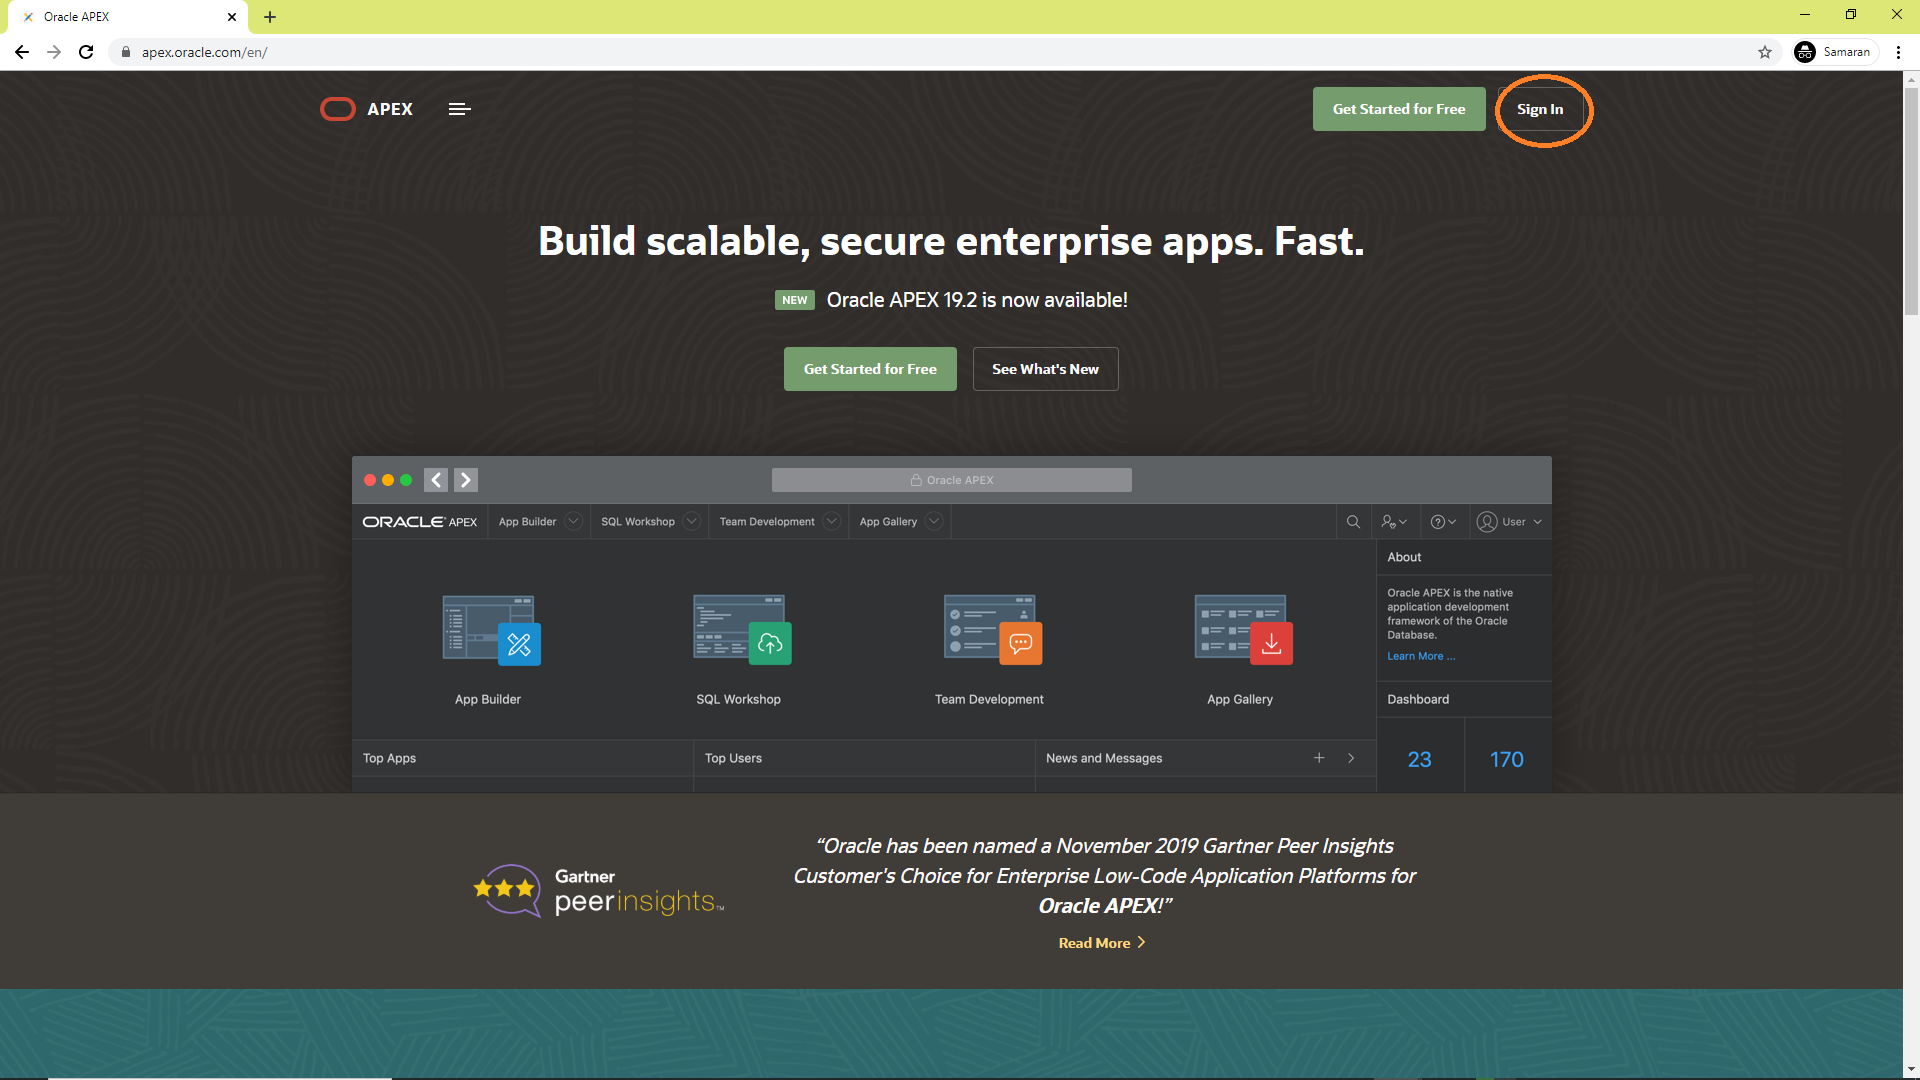
\includegraphics[scale=0.23]{figures/1.png}
        \caption{\textit{Halaman APEX.ORACLE.COM}}
        \end{center}
        \end{figure}
        
        
        \begin{figure}[!htbp]
        \item[2]Pada Halaman Login Klik Request a Workspace, karena kita belum mempunyai akun kita akan regristrasi terlebih dahulu, pada form yang di gambar yaitu form untuk login untuk memasuki halaman aplikasi kita yang saat kita buat nanti,  lihat pada Gambar 2.2.
        \begin{center}
        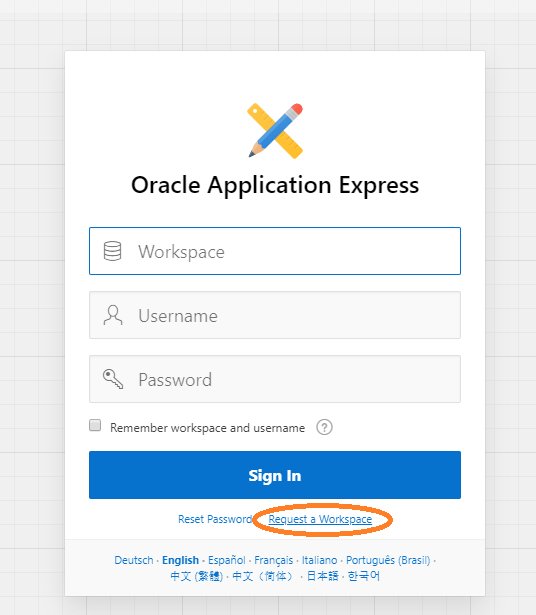
\includegraphics[scale=0.5]{figures/2.png}
        \caption{\textit{Req Workspace}}
        \end{center}
        \end{figure}
        
        \begin{figure}[!htbp]
        \item[3]Isikan data diri anda dengan benar ,lihat pada Gambar 2.3, First Name = Isikan Nama Depan Anda, Last Name = Isikan Nama Belakang Anda, Email = Isikan Email Anda (Wajib karena saat mengisi semua form regristrasi nanti akan diberikan notifikasi melalui email, Workspace = Nama Proyek yang akan dibuat.
        \begin{center}
        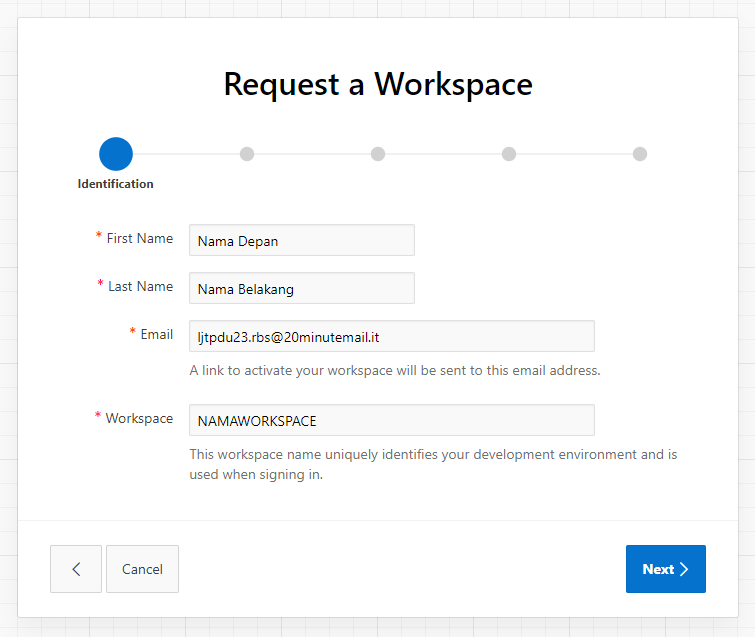
\includegraphics[scale=0.5]{figures/3.png}
        \caption{\textit{Req Workspace2}}
        \end{center}
        \end{figure}
        
        \begin{figure}[!htbp]
        \item[4]Berikut adalah Survey dimana oracle akan memastikan anda menggunakan dengan baik aplikasi yang akan anda kembangkan , pertama oracle akan menanyakan "Apakah anda pengguna baru Oracle Application Express?", dan yang kedua "Apakah kamu mempunyai plan menggunakan proyek ini untuk universitas atau pelatihan ?", isilah data data berikut seperti Gambar 2.4.
        \begin{center}
        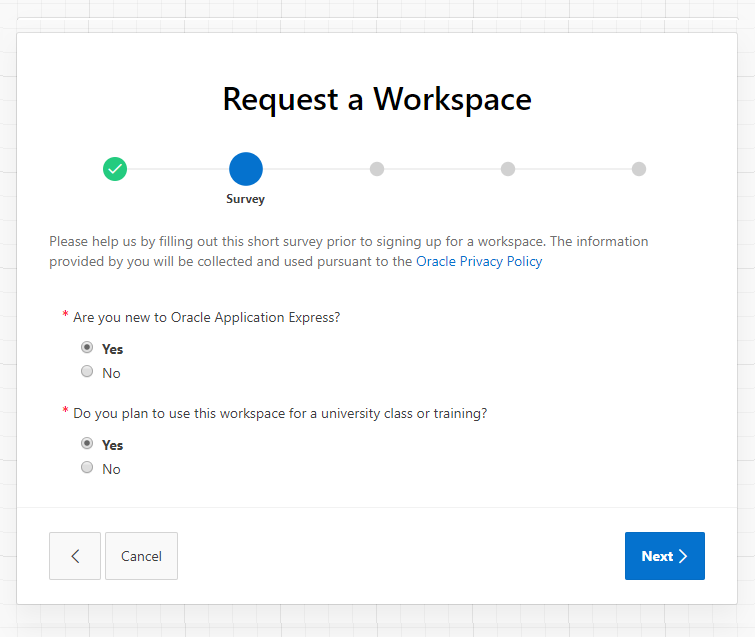
\includegraphics[scale=0.5]{figures/4.png}
        \caption{\textit{Req Workspace3}}
        \end{center}
        \end{figure}
        
        \begin{figure}[!htbp]
        \item[5]Form berikut adalah form justification atau pembenaran, atau melihat apakah anda robot atau tidak oracle akan menanyakan "Mengapa anda ingin meminta akses serfis ini ?" isikan form berikut bebas dengan kata-kata yang anda sukai, lihat pada Gambar 2.5.
        \begin{center}
        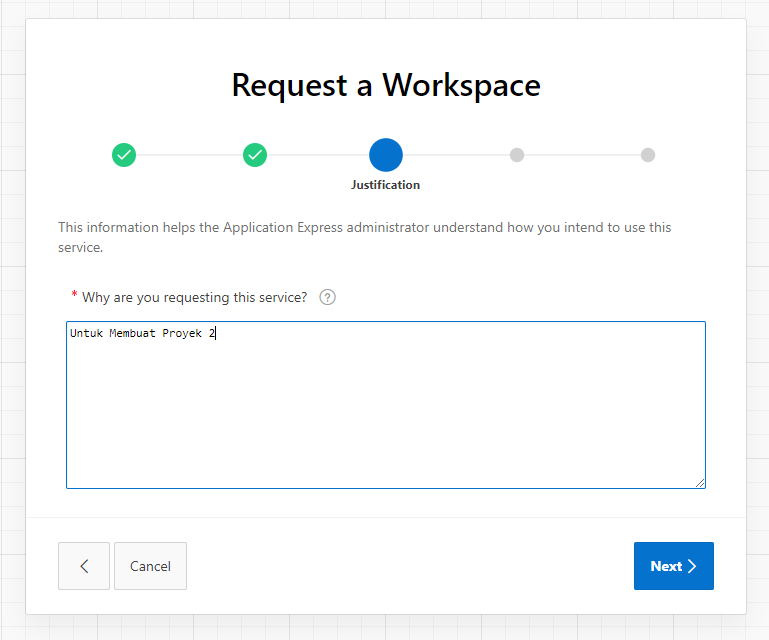
\includegraphics[scale=0.5]{figures/5.png}
        \caption{\textit{Req Workspace4}}
        \end{center}
        \end{figure}
        
        \begin{figure}[!htbp]
        \item[6]Berikut adalah step form Persetujuan, oracle akan menanyakan apakah kamu akan menyetujui semua persetujuan menggunakan aplikasi, jika anda setuju centang "I accept the terms", lihat pada Gambar 2.6.
        \begin{center}
        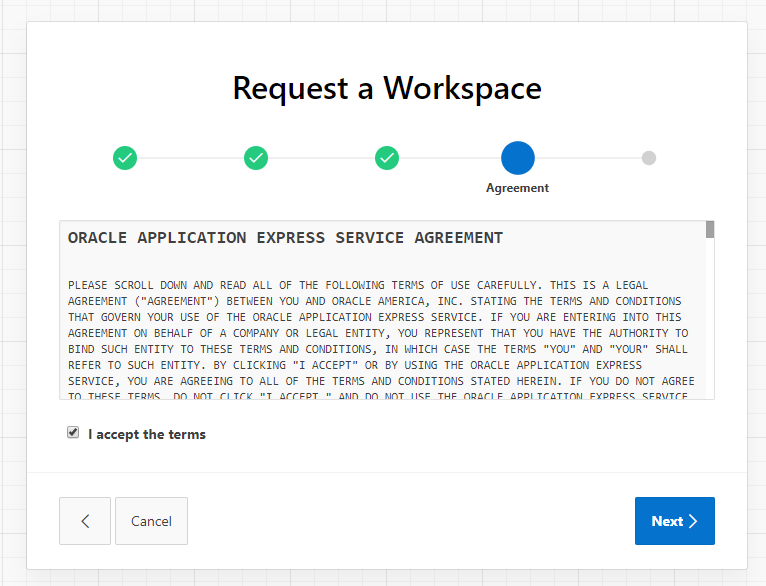
\includegraphics[scale=0.5]{figures/6.png}
        \caption{\textit{Req Workspace5}}
        \end{center}
        \end{figure}

        \begin{figure}[!htbp]
        \item[7]Berikut adalah step form Konfirmasi apakah data yang anda inputkan sudah benar jika semua sudah benar klik Submit Request, lihat pada Gambar 2.7.
        \begin{center}
        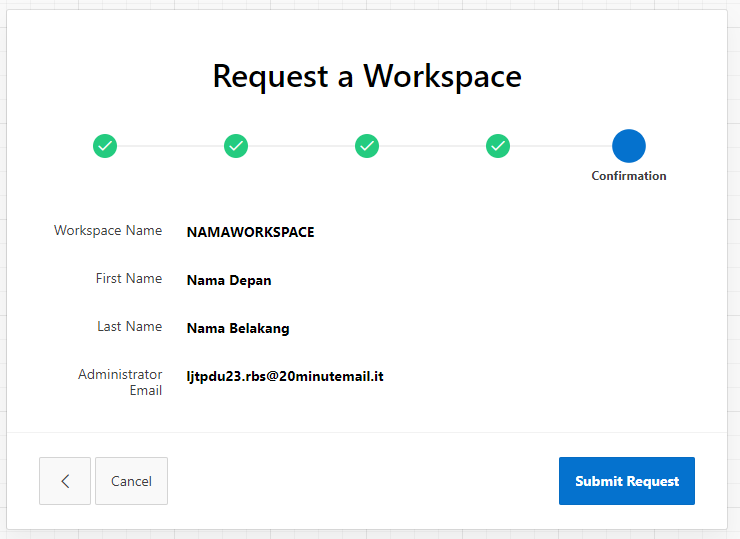
\includegraphics[scale=0.5]{figures/7.png}
        \caption{\textit{Req Workspace6}}
        \end{center}
        \end{figure}
        
        \begin{figure}[!htbp]
        \item[8]Permintaan membuat projek telah terkirim, anda akan menerima email yang anda inputkan saat mengisi form Regristrasi tadi, segera cek email anda, kalau belum di terima biasanya akan ada waktu interval 0-15 menit, karena oracle akan mengidentifikasi form yang anda inputkan tadi,lihat pada Gambar 2.8.
        \begin{center}
        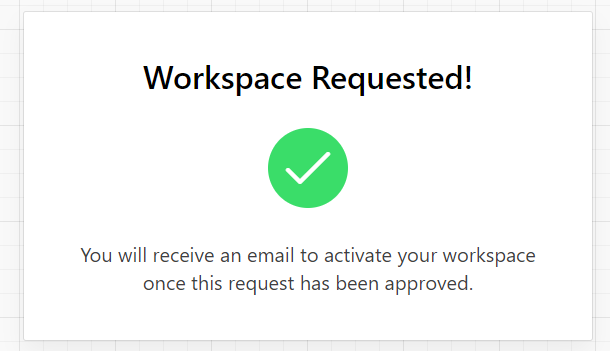
\includegraphics[scale=0.5]{figures/8.png}
        \caption{\textit{Req Workspace7}}
        \end{center}
        \end{figure}
        
        \begin{figure}[!htbp]
        \item[9]Saat anda menerima email seperti berikut dengan data data yang anda inputkan pada form tadi seperti Workspace dan Username, lalu anda akan menerima link untuk environment, setelah semua dirasa benar klik tombol "Create Workspace", lihat pada Gambar 2.9.
        \begin{center}
        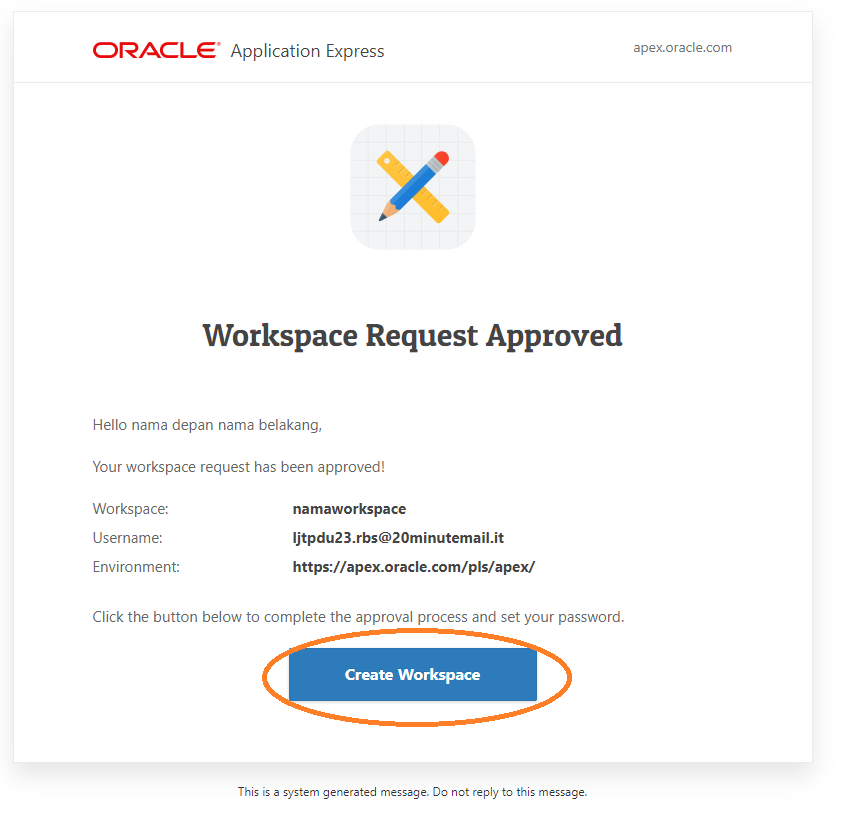
\includegraphics[scale=0.5]{figures/9.png}
        \caption{\textit{Cek Email}}
        \end{center}
        \end{figure}
        
        \begin{figure}[!htbp]
        \item[10]Selamat Workspace anda telah dibuat ! , anda akan diberitahu notifikasi tersebut , lalu selanjutnya anda lakukan Continue to Sign In Screen, lihat pada Gambar 2.10.
        \begin{center}
        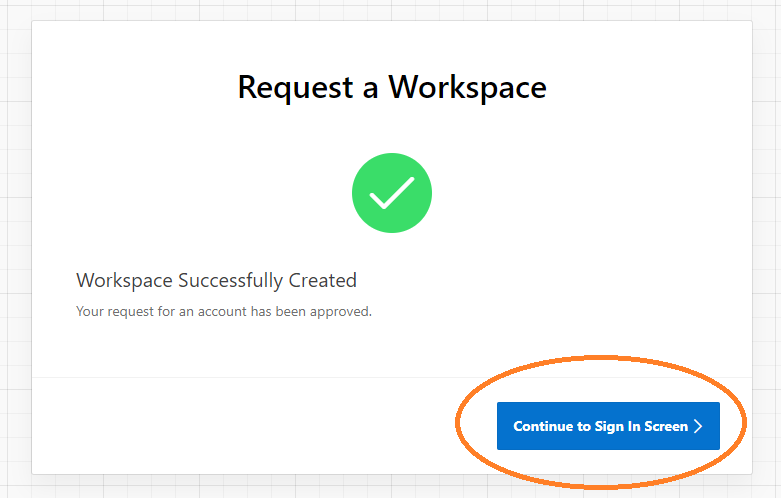
\includegraphics[scale=0.5]{figures/10.png}
        \caption{\textit{Continue to Sign In Screen}}
        \end{center}
        \end{figure}
        
        \begin{figure}[!htbp]
        \item[11]Lalu anda akan dialihkan pada halaman untuk mengganti password untuk workspace anda, Masukkan password anda yg diinginkan dan konfirmasi password ke 2 secara benar, lalu klik Apply Changes, lihat pada Gambar 2.11.
        \begin{center}
        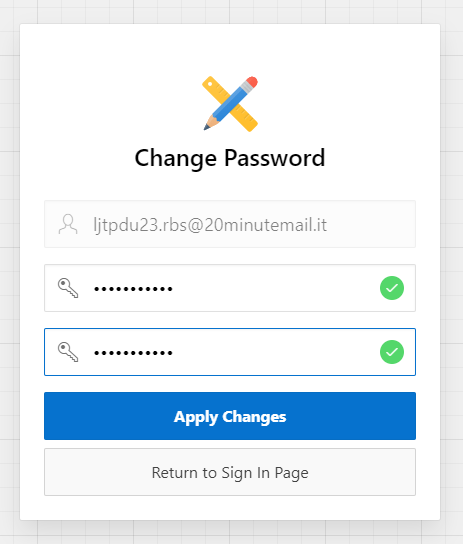
\includegraphics[scale=0.5]{figures/11.png}
        \caption{\textit{Masukan Password}}
        \end{center}
        \end{figure}
        
        \begin{figure}[!htbp]
        \item[12]Jika sudah membuat password, anda akan dialihkan pada halaman utama Aplikasi Oracle Apex, yang dimana anda akan membuat aplikasi, lihat pada Gambar 2.12.
        
        \begin{itemize}
            \item App Builder = Untuk membuat dan mengelola aplikasi web, pastikan database sudah ada.
            \item SQL Workshop = Untuk membuat dan mengelola Database, setiap informasi biasanya tertuju pada SQL Workspace.
            \item  Team Development = adalah aplikasi bawaan yang dikelola oleh APEX, namun kita tidak akan menggunakan fitur ini.
            \item App Gallery = Untuk membuat aplikasi yang sudah ada atau sudah jadi untuk dimasukkan ke workspace kita, namun kita tidak akan menggunakan fitur ini.
        \end{itemize}
        \par Pada panel sebelah kiri anda akan dijelaskan tentang apa itu Oracle Apex, Dashboard yang berisi berapa banyak Aplikasi anda, Tables berapa banyak jumlah tabel.
        \par Lalu ada Site Specific Task yaitu website yang akan mengalihkan pada suatu guide atau yang membahas  tentang Oracle APEX,
        \par Lalu Resources, adalah halaman komunitas-komunitas yang telah diremiskan oleh Oracle Apex.
        \par Tab Social, adalah halaman social Oracle Apex yang sering dijumpai.
        \begin{center}
        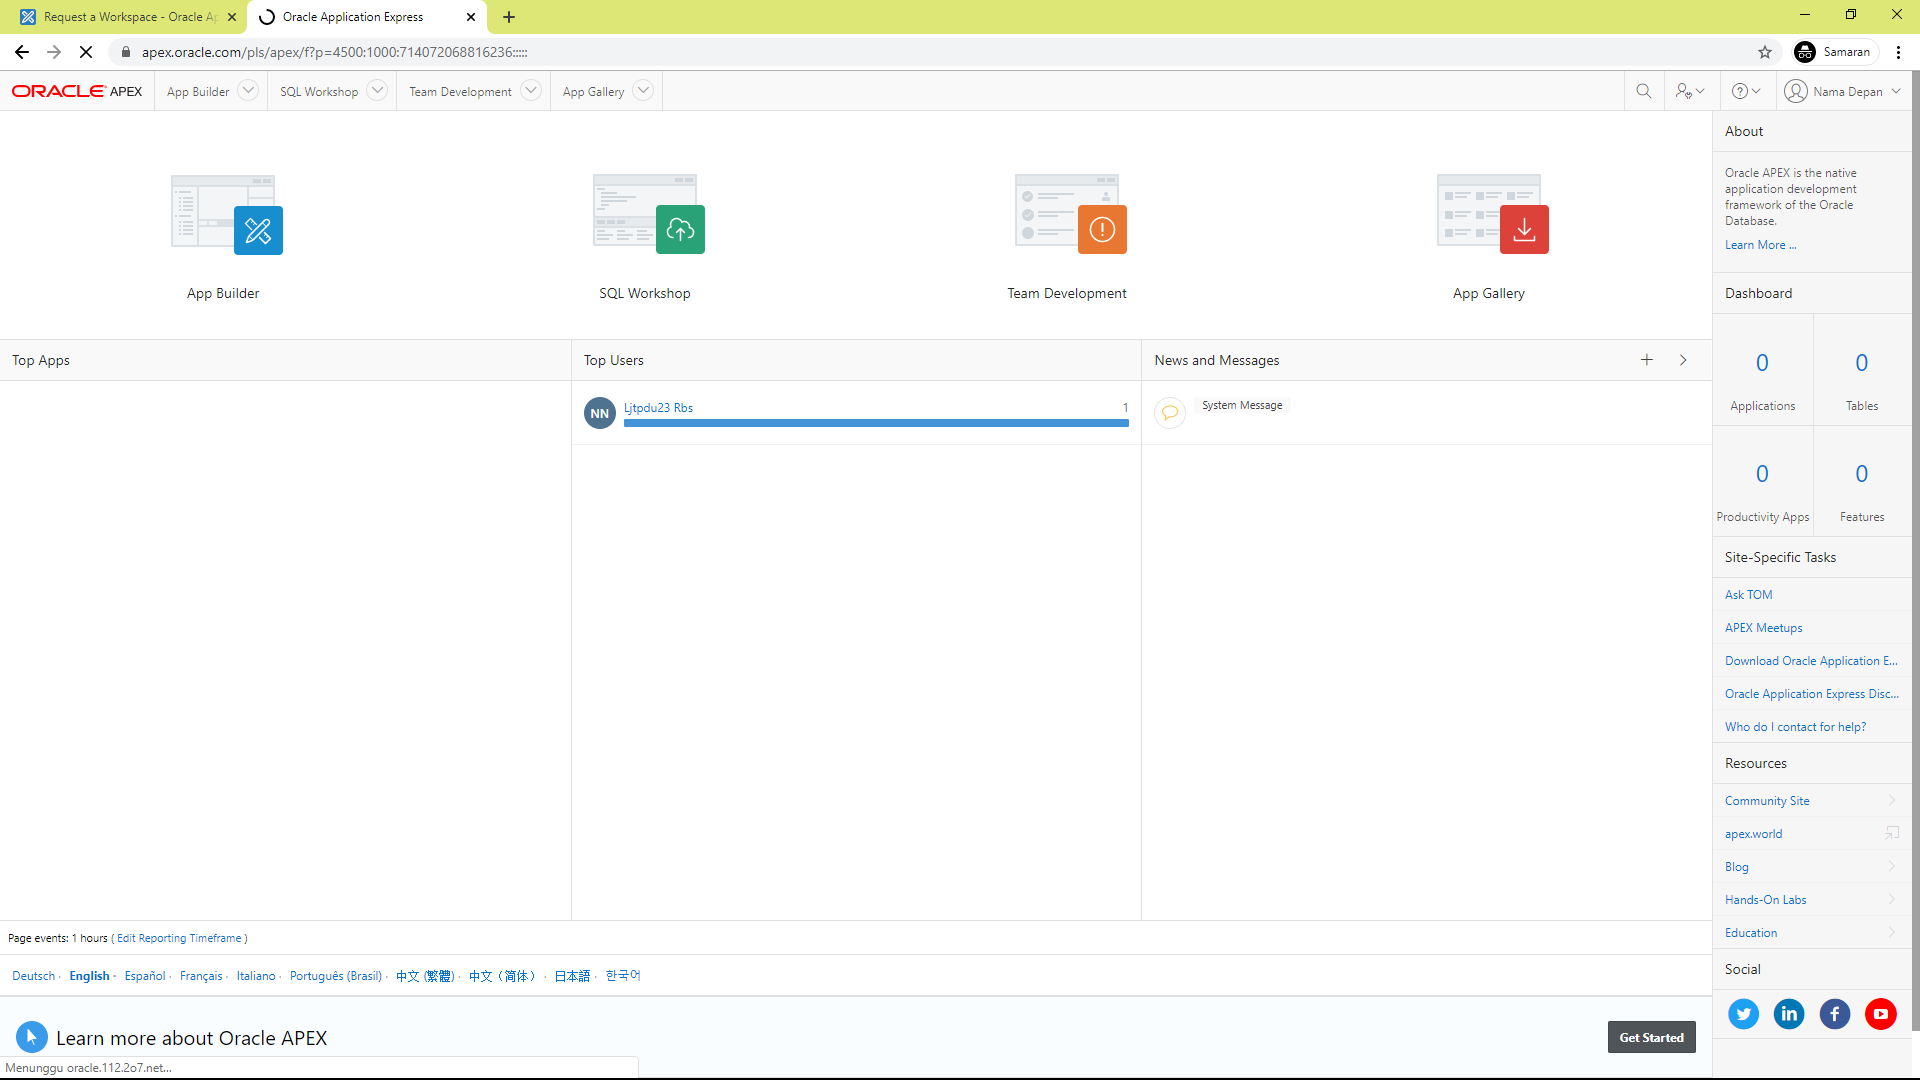
\includegraphics[scale=0.23]{figures/12.png}
        \caption{\textit{Halaman Utama Apex}}
        \end{center}
        \end{figure}
\end{itemize}

\chapter{Menyiapkan Tabel Database dan Merelasikannya}
\section{Pendahuluan}
Dengan membuat tabel berfungsi agar aplikasi terhubung dengan database, dalam buku ini kita akan membuat beberapa tabel yang saling berelasi, tabel ini mempunyai atribut yang dimiliki pada data yang mengacu pada aplikasi.

\subsection{Definisi Database Menurut Para Ahli}
Kemampuan basis data Oracle dapat bekerja pada banyak platform merupakan salah satu  fasilitas  yang dimanfaatkan untuk  menyimpan data dengan membuat sub routine sehinggadalam  melakukan eksekusi data menjadi  cepat \cite{pemanfaatandatabase2018}.

\par Oracle merupakan sebuah sistem manajemen basis data yang dikenal memiliki fitur dan kecanggihan yang membuat pengelolaan basis data menjadi efisien dan efektif. Namun perancangan basis data yang diterapkan pada suatu sistem manajemen basis data tidak kalah pentingnya. Perancangan basis data yang baik akan mempermudah implementasi aplikasi serta mengoptimalkan kinerja dari sistem manajemen basis data itu sendiri\cite{perancanganDB2013}.

\par Pengolahan data untuk menghasilkan informasi secara terkomputerisasi, merupakan sarana yang sangat dibutuhkan saat ini pada berbagai jenis usaha, karena informasi mampudisajikan dalam waktu yang cepat dan akurat. Informasi yang mampu disajikan dengancepat dan akurat mampu menghasilkan pengambilan keputusan yang cepat dan efektif\cite{jurnalDB2011}.

\section{Siapkan Tabel}
Dalam pembuatan tabel kita siapkan 7 tabel untuk mengelola aplikasi absensi pada buku ini yaitu :
\begin{itemize}
    \item[1]JABATAN\_ORMAWA
            \begin{itemize}
                \item KODE\_JABATAN (NUMBER) PK
                \item JABATAN (VARCHAR2(50))
            \end{itemize}
    \item[2]JURUSAN
            \begin{itemize}
                \item KODE\_JURUSAN (NUMBER) PK
                \item NAMA\_JURUSAN (VARCHAR2(255))
            \end{itemize}
    \item[3]ORMAWA
            \begin{itemize}
                \item KODE\_ORMAWA (VARCHAR2(255)) PK
                \item NAMA\_ORMAWA (VARCHAR2(255))
            \end{itemize}
    \item[4]RUANGAN
            \begin{itemize}
                \item ID\_RUANGAN (NUMBER) PK
                \item JENIS\_RUANGAN (VARCHAR2(255))
            \end{itemize}
    \item[5]STAFF\_BAAK
            \begin{itemize}
                \item NIK (NUMBER) PK
                \item NAMA\_STAFF (VARCHAR2(255))
                \item NO\_TELP (VARCHAR2(20))
                \item JABATAN (VARCHAR2(30))
            \end{itemize}
    \item[6]MAHASISWA
            \begin{itemize}
                \item NPM (NUMBER) PK
                \item NAMA (VARCHAR2(255))
                \item KELAS (VARCHAR2(255))
                \item KODE\_ORMAWA (VARCHAR2(255)) FK
                \item NO\_TELP\_MHS (VARCHAR2(14))
                \item KODE\_JURUSAN (NUMBER) FK
                \item KODE\_JABATAN (NUMBER) FK
            \end{itemize}
    \item[7]PEMINJAMAN\_RUANGAN
            \begin{itemize}
                \item ID\_PEMINJAMAN (NUMBER)
                \item NPM (NUMBER) FK
                \item ID\_RUANGAN (NUMBER) FK
                \item NIK (NUMBER) FK
                \item TANGGAL (DATE)
                \item JAM\_AWAL (VARCHAR2(4000))
                \item JAM\_AKHIR (VARCHAR2(4000))
                \item STATUS\_PEMINJAMAN (VARCHAR2(4000))
            \end{itemize}
    \par KETERANGAN :
            \begin{itemize}
                \item NUMBER = Tipe Data Sebagai NOMER/ANGKA
                \item DATE = Tipe Data Sebagai TANGGAL
                \item VARCHAR2 = Tipe Data Sebagai NOMER/ANGKA/SIMBOL
                \item PK = Primary Key, Kunci Utama/Unik Untuk Merelasikan Antar Tabel
                \item FK = Foreign Key, Kunci Kedua/Kunci Asing untuk merelasikan dari kunci unik/Primary Key
            \end{itemize}
    
        \begin{figure}
        \par Lalu merelasikannya seperti Gambar berikut :
        \begin{center}
        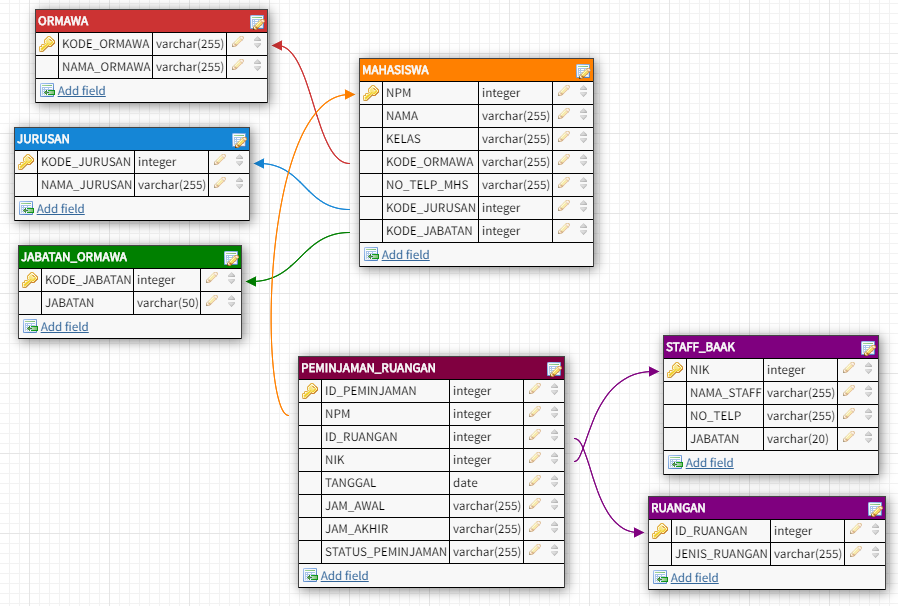
\includegraphics[scale=0.45]{figures/TABEL.png}
        \caption{\textit{TABEL DATABASE}}
        \end{center}
        \end{figure}
\end{itemize}

\chapter{Membuat QUERY Tabel}
\section{Membuka SQL Command Atau CLI}
Setelah database telah disiapkan dan direlasikan kita akan membuat query setiap tabel, pertama tama buka kembali aplikasi ORACLE APEX Online anda lalu pilih SQL Workshop.
\begin{itemize}
    \item[1] Buka SQL Workshop pada Oracle Apex Online Anda,lihat Gambar 4.1.
    \item[2] Buka SQL Command pada Oracle Apex Online Anda,lihat Gambar 4.2.
    \item[3] Anda akan menjumpai seperti CLI Database, disitu anda akan membuat query yang nanti akan dijelaskan pada buku ini, lalu pada tab bawah amda akan menjumpai :
    \par Results (Untuk Hasil Dari Query), Explain (Adalah Penjelasan Jika Query Salah), Describe (Untuk Describe Sebuah Objek), Saved SQL (Me-nampilkan data SQL yangg tersimpan), History (Menampilkan Query Yang Pernah Di Run Sebelumnya),lihat Gambar 4.3.      
\end{itemize}

\begin{figure}
        \begin{center}
        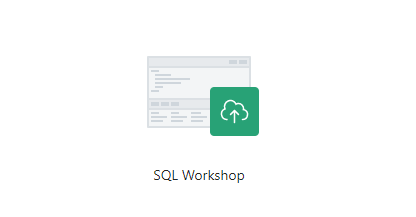
\includegraphics[scale=0.5]{figures/sql_wksp.png}
        \caption{\textit{SQL Workshop}}
        \end{center}
        \end{figure}
        
\begin{figure}
        \begin{center}
        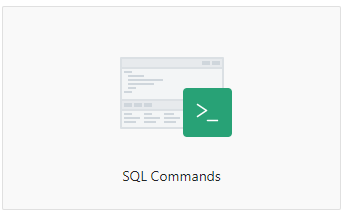
\includegraphics[scale=0.5]{figures/sql_command.png}
        \caption{\textit{SQL Command}}
        \end{center}
        \end{figure}
\begin{figure}
       
        \begin{center}
        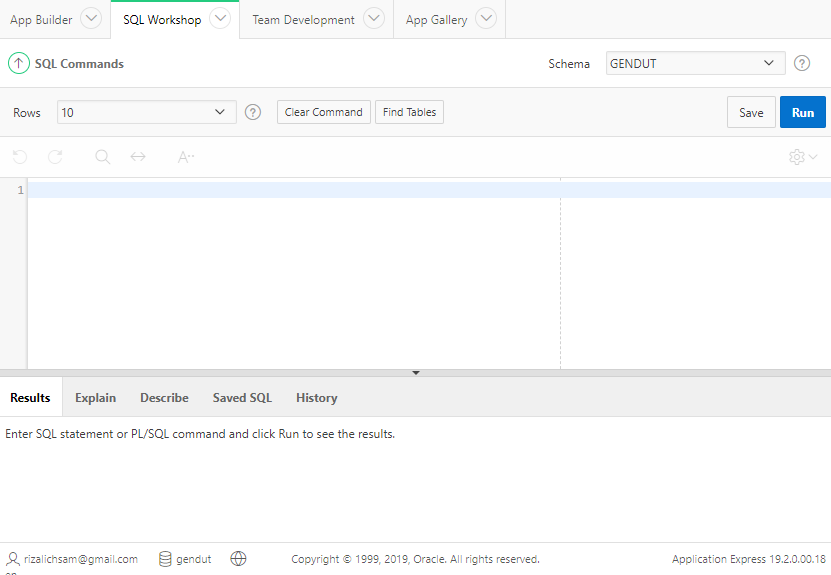
\includegraphics[scale=0.5]{figures/sql_command2.png}
        \caption{\textit{Isi SQL Command}}
        \end{center}
        \end{figure}

\section{Membuat Query}
setelah membuka SQL Command buku ini akan menjelaskan Query dari setiap tabel yang telah direlasikan sebelumnya,berikut adalah penjelasannnya :

\begin{itemize}
    \item Query pada tabel JABATAN\_ORMAWA
            \begin{lstlisting}
/*RUN QUERY PERTAMA*/

CREATE TABLE  "JABATAN_ORMAWA" 
("KODE_JABATAN" NUMBER,
"JABATAN" VARCHAR2(50), 
PRIMARY KEY ("KODE_JABATAN")
USING INDEX  ENABLE
)
/

/*RUN QUERY KEDUA*/

CREATE OR REPLACE EDITIONABLE TRIGGER  "JABATAN_TRG" 
BEFORE INSERT ON JABATAN_ORMAWA 
FOR EACH ROW
BEGIN
  SELECT JABATAN_SEQ.NEXTVAL
  INTO   :new.KODE_JABATAN
  FROM   dual;
END;
/

/*RUN QUERY KETIGA*/

ALTER TRIGGER  "JABATAN_TRG" ENABLE
/
            \end{lstlisting}
    \item Query pada tabel JURUSAN
            \begin{lstlisting}
CREATE TABLE  "JURUSAN" 
   (	"KODE_JURUSAN" NUMBER NOT NULL ENABLE, 
	"NAMA_JURUSAN" VARCHAR2(255) NOT NULL ENABLE, 
	 PRIMARY KEY ("KODE_JURUSAN")
  USING INDEX  ENABLE
   )
/
            \end{lstlisting}
    \item Query pada tabel ORMAWA
            \begin{lstlisting}
CREATE TABLE  "ORMAWA" 
   (	"KODE_ORMAWA" VARCHAR2(255) NOT NULL ENABLE, 
	"NAMA_ORMAWA" VARCHAR2(255) NOT NULL ENABLE, 
	 PRIMARY KEY ("KODE_ORMAWA")
  USING INDEX  ENABLE
   )
/
            \end{lstlisting}
        
        \item Query pada tabel RUANGAN
            \begin{lstlisting}
CREATE TABLE  "RUANGAN" 
   (	"ID_RUANGAN" NUMBER(*,0) NOT NULL ENABLE, 
	"JENIS_RUANGAN" VARCHAR2(255) NOT NULL ENABLE, 
	 PRIMARY KEY ("ID_RUANGAN")
  USING INDEX  ENABLE
   )            
            \end{lstlisting}
\item Query pada tabel STAFF\_BAAK
            \begin{lstlisting}
CREATE TABLE  "STAFF_BAAK" 
   (	"NIK" NUMBER(*,0) NOT NULL ENABLE, 
	"NAMA_STAFF" VARCHAR2(255), 
	"NO_TELP" VARCHAR2(20), 
	"JABATAN" VARCHAR2(30), 
	 PRIMARY KEY ("NIK")
  USING INDEX  ENABLE
   )
/
            \end{lstlisting}
\item Query pada tabel MAHASISWA
            \begin{lstlisting}
/* RUN QUERY PERTAMA */

CREATE TABLE  "MAHASISWA" 
   (	"NPM" NUMBER(*,0) NOT NULL ENABLE, 
	"NAMA" VARCHAR2(255) NOT NULL ENABLE, 
	"KELAS" VARCHAR2(255) NOT NULL ENABLE, 
	"KODE_ORMAWA" VARCHAR2(255) NOT NULL ENABLE, 
	"NO_TELP_MHS" VARCHAR2(14), 
	"KODE_JURUSAN" NUMBER, 
	"KODE_JABATAN" NUMBER, 
	 PRIMARY KEY ("NPM")
  USING INDEX  ENABLE
   )
/

/* RUN QUERY KEDUA */

ALTER TABLE  "MAHASISWA" ADD CONSTRAINT "FK_JABATAN" FOREIGN KEY ("KODE_JABATAN")
	  REFERENCES  "JABATAN_ORMAWA" ("KODE_JABATAN") ENABLE
/

/* RUN QUERY KETIGA */

ALTER TABLE  "MAHASISWA" ADD CONSTRAINT "FK_JURUSAN" FOREIGN KEY ("KODE_JURUSAN")
	  REFERENCES  "JURUSAN" ("KODE_JURUSAN") ENABLE
/

/* RUN QUERY KEEMPAT */

ALTER TABLE  "MAHASISWA" ADD CONSTRAINT "FK_ORMAWA" FOREIGN KEY ("KODE_ORMAWA")
	  REFERENCES  "ORMAWA" ("KODE_ORMAWA") ENABLE
/
            
            \end{lstlisting}
\item Query pada tabel PEMINJAMAN\_RUANGAN
            \begin{lstlisting}
/* RUN QUERY PERTAMA */

CREATE TABLE  "PEMINJAMAN_RUANGAN" 
   (	"ID_PEMINJAMAN" NUMBER GENERATED ALWAYS AS IDENTITY MINVALUE 1 MAXVALUE 999999999999 INCREMENT BY 1 START WITH 1 CACHE 20 NOORDER  NOCYCLE  NOKEEP  NOSCALE  NOT NULL ENABLE, 
	"NPM" NUMBER, 
	"ID_RUANGAN" NUMBER, 
	"NIK" NUMBER, 
	"TANGGAL" DATE, 
	"JAM_AWAL" VARCHAR2(4000), 
	"JAM_AKHIR" VARCHAR2(4000), 
	"STATUS_PEMINJAMAN" VARCHAR2(4000), 
	 PRIMARY KEY ("ID_PEMINJAMAN")
  USING INDEX  ENABLE
   )
/
/* RUN QUERY KEDUA */

ALTER TABLE  "PEMINJAMAN_RUANGAN" ADD CONSTRAINT "FK_NIK" FOREIGN KEY ("NIK")
	  REFERENCES  "STAFF_BAAK" ("NIK") ENABLE
/
/* RUN QUERY KETIGA */

ALTER TABLE  "PEMINJAMAN_RUANGAN" ADD CONSTRAINT "FK_NPM" FOREIGN KEY ("NPM")
	  REFERENCES  "MAHASISWA" ("NPM") ENABLE
/

/* RUN QUERY KEEMPAT */

ALTER TABLE  "PEMINJAMAN_RUANGAN" ADD CONSTRAINT "FK_RUANGAN" FOREIGN KEY ("ID_RUANGAN")
	  REFERENCES  "RUANGAN" ("ID_RUANGAN") ENABLE
/
            
            \end{lstlisting}

\end{itemize}


\chapter{Membuat Fungsi Trigger dan Sequence}
\section{Pengertian Trigger}
Trigger adalah blok PL/SQL yang disimpan dalam database dan akan diaktivasi ketika kita melakukan statement-statement SQL (DELETE, UPDATE, dan INSERT) pada sebuah tabel. Aktivasi trigger didasarkan pada event yang terjadi di dalam tabel tersebut sehingga trigger dapat membantu dalam menjaga integritas dan konsistensi data.
\par Implementasi trigger yang sering ditemui dalam dunia nyata adalah untuk mengeset dan mengubah nilai kolom dalam suatu tabel sehingga validasi nilai dari tabel tersebut akan terjaga. Adanya trigger dalam database akan meringankan kita dalam pembuatan aplikasi karena di dalam aplikasi yang kita buat, kita tidak perlu lagi untuk melakukan validasi data.
\par Dalam trigger Oracle telah menyediakan statement CREATE TRIGGER untuk membuat
sebuah trigger yang selanjutnya akan diaktivasi berdasarkan event tertentu. Secara
umum, event trigger terbagi menjadi dua, yaitu BEFORE (sebelum) dan AFTER
(setelah). Event tersebut menandakan kapan trigger akan diaktivasi, apakah sebelum
ataukah sesudah proses yang dilakukan di dalam tabel bersangkutan\cite{mudafiq2003trigger}.
\begin{table}[]
    \begin{center}
\begin{tabular}{ |c|c| } 
 \hline
 Nama Event & Keterangan  \\ \hline 
 BEFORE INSERT & Diaktifkan sekali sebelum Statement INSERT  \\ \hline
 AFTER INSERT & Diaktifkan sekali setelah Statement INSERT  \\ \hline
 BEFORE UPDATE & Diaktifkan sekali sebelum Statement UPDATE \\ \hline
 AFTER UPDATE & Diaktifkan sekali setelah Statement UPDATE \\ \hline
 BEFORE DELETE & Diaktifkan sekali sebelum Statement DELETE \\ \hline
 AFTER DELETE & Diaktifkan sekali setelah Statement DELETE \\
 \hline
\end{tabular}
\caption{Tabel Pengertian Trigger}
    \label{tabel_kebutuhan_sistem}
\end{center}
\end{table}
\section{Pengertian Sequence}
Sequence iaalah salah satu object yang ada di aplikasi Oracle Apex pada database yang digunakan untuk melakukan penomoran otomatis. Namun pada database MySQL yang biasa lebih dikenal dengan nama Auto Increment, Sequence biasanya digunakan sebagai Primary Key untuk membuat ID yang secara otomatis terinput oleh database.
\par pada Oracle Apex database, anda dapat membuat sequence hingga mencapai kelipatan yang tak terbatas, namun anda juga bisa mengaturnya dengan sesuai kebutuhan anda.

\section{Membuat Query Sequence dan Trigger}
Dalam tahap ini yaitu kita akan membuat Query pada SQL Command, tuliskan kode kode berikut

\begin{itemize}
    \item[1] Buat Query Untuk Sequence terlebih dahulu yang nanti akan di integrasikan pada Trigger JABATAN\_TRG
    \begin{lstlisting}
CREATE SEQUENCE   "JABATAN_SEQ"  
 MINVALUE 1 
 MAXVALUE 9999999999999999999999999999 
 NOCYCLE
 CACHE 20
 NOORDER;
    \end{lstlisting}
    \item[2] Buat Query TRIGGER yang nanti akan terhubung pada tabel JABATAN
    \begin{lstlisting}
/*QUERY PERTAMA*/

CREATE OR REPLACE EDITIONABLE TRIGGER  "JABATAN_TRG" 
BEFORE INSERT ON JABATAN_ORMAWA 
FOR EACH ROW

BEGIN
  SELECT JABATAN_SEQ.NEXTVAL
  INTO   :new.KODE_JABATAN
  FROM   dual;
END;

/

/*QUERY KEDUA*/

ALTER TRIGGER  "JABATAN_TRG" ENABLE
/
    \end{lstlisting}
 \end{itemize}


\chapter{Membuat View Tabel Beserta Join Tabel}
\section{Pengertian View dalam Database}
Di dalam Oracle SQL, View dapat didefenisikan sebagai tabel virtual yang tidak dapat di ubah isi datanya. Tabel ini bisa berasal dari tabel lain, atau bisa gabungan dari beberapa tabel.
\par Tujuan dari pembuatan VIEW sebuah query ialah untuk kenyamanan developer dalam mempermudah penulisan query sql, untuk keamanan (menyembunyikan beberapa kolom yang bersifat rahasia atau tidak boleh diketahui user lain), atau dalam beberapa case bisa digunakan untuk mempercepat suatu proses dalam menampilkan data (jika kita akan menjalankan query tersebut secara berulang).

\subsection{Contoh Query View}
Berikut adalah contoh dari query dari View, dalam beberapa kasus banyak orang mengartikan view sebagai query yang sangat simpel, contohnya :
\begin{itemize}
    \item Query yang pertama dibutuhkan 
\begin{lstlisting}
CREATE VIEW ... AS ... ;
\end{lstlisting}
    \item Atau anda dapat menambahkan REPLACE
\begin{lstlisting}
CREATE OR REPLACE VIEW ... AS ... ;
\end{lstlisting}
    \item Sebagai Contoh Membuat View Dari Tabel MAHASISWA
\begin{lstlisting}
CREATE OR REPLACE VIEW TBL_MHS AS
SELECT * FROM MAHASISWA;
\end{lstlisting}
    \item Dan untuk menghapusnya cukup seperti berikut
\begin{lstlisting}
DROP VIEW TBL_MHS;
\end{lstlisting}
\end{itemize}

\section{Pengertian Join Dalam Database}
Join adalah sebutan untuk menggabungkan 1 tabel antara 2 atau tabel lainnya yang berelasi antar primary key atau foreign key, biasanya Query join untuk menampilkan suatu data yang penting dalam beberapa tabel lalu menggabungkannya agar seakan akan data dari satu tabel dengan tabel lainnya tersambung, dapat dicontohkan sebagai berikut :

\begin{itemize}
    \item Menggabungkan 1 tabel dengan 2 tabel lainnya yaitu dari tabel MAHASISWA dan yang akan bergabung pada tabel tersebut yaitu tabel JURUSAN dan JABATAN\_ORMAWA.
    \begin{lstlisting}
SELECT M.NPM,M.NAMA,M.KELAS,M.KODE_JURUSAN,J.NAMA_JURUSAN,M.KODE_ORMAWA,M.KODE_JABATAN,O.JABATAN,M.NO_TELP_MHS
FROM MAHASISWA M
INNER JOIN JURUSAN J
    on M.KODE_JURUSAN = J.KODE_JURUSAN
INNER JOIN JABATAN_ORMAWA O
    on M.KODE_JABATAN = O.KODE_JABATAN
    \end{lstlisting}
\end{itemize}

\section{Menggabungkan Query View dengan Join}
Dalam penggabungan query view dengan join anda dapat melakukan cara berikut yaitu, membuat nama View yaitu DATA\_MHS, lalu membberikan select dari join tabel MAHASISWA dan yang akan bergabung pada tabel tersebut yaitu tabel JURUSAN dan JABATAN\_ORMAWA.
\par Berikut adalah contohnya :
    \begin{lstlisting}
CREATE OR REPLACE VIEW DATA_MHS AS 
  SELECT M.NPM,M.NAMA,M.KELAS,M.KODE_JURUSAN,J.NAMA_JURUSAN,M.KODE_ORMAWA,M.KODE_JABATAN,O.JABATAN,M.NO_TELP_MHS
FROM MAHASISWA M
INNER JOIN JURUSAN J
    on M.KODE_JURUSAN = J.KODE_JURUSAN
INNER JOIN JABATAN_ORMAWA O
    on M.KODE_JABATAN = O.KODE_JABATAN
    \end{lstlisting}

\chapter{Membuat Aplikasi Pada App Builder}
\section{Tahapan Cara Membuat Aplikasi}
Berikut Adalah Tahapan Cara membuat aplikasi, dengan menuju halaman utama aplikasi Oracle APEX anda akan mendapati App Builder yang berfungsi untuk membuat aplikasi WEB atau disebut Web Based Application dengan perantara host yang disediakan oleh Oracle APEX.

\par pada saat membuat aplikasi web caranya sangat mudah seperti kita hanya akan mendrag dan drop, namun ada juga yang harus pakai koding html/css untuk menambah fitur lainnya, langsung saja cek di bawah ini.
   
\begin{itemize}
        \begin{figure}[!htbp]
        \item[1]Pilih Create App.
        \begin{center}
        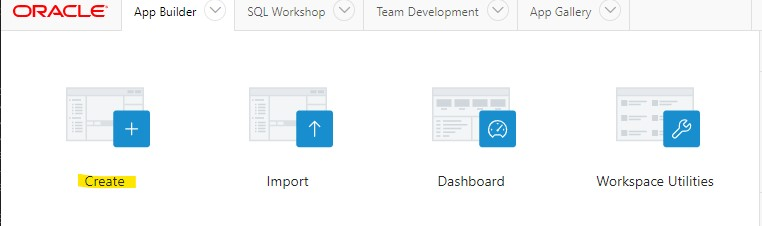
\includegraphics[scale=0.4]{figures/create_app.jpg}
        \caption{\textit{Create App}}
        \end{center}
        \par Pada tahapan ini anda akan diberikan 4 pilihan yaitu :
        \begin{itemize}
            \item Create = Untuk membuat Aplikasi (Pilih yang ini)
            \item Import = Untuk mengimpor aplikasi yang sudah ada/jadi
            \item Dashboard = melihat dasbor aplikasi yang sudah ada
            \item Workspace Utilities = Utiliti Workspace
        \end{itemize}
        \end{figure}
        
        \begin{figure}[!htbp]
        \item[2]Pilih New Application 
        \begin{center}
        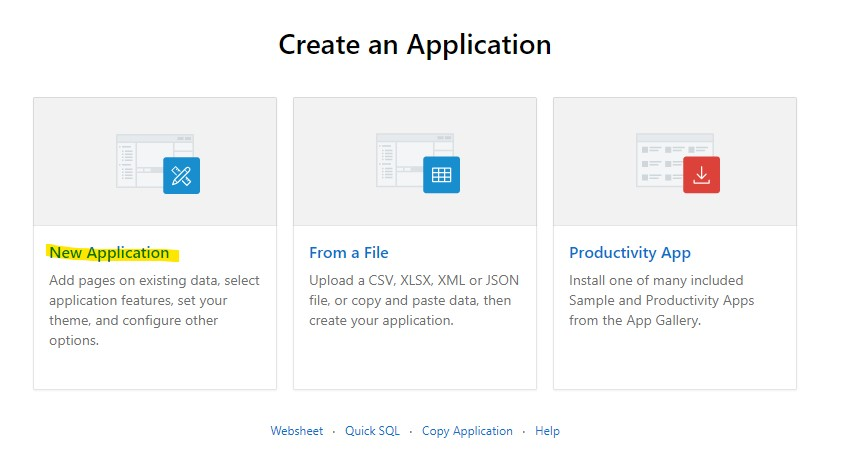
\includegraphics[scale=0.5]{figures/create_a_new_application.jpg}
        \caption{\textit{Pilih New Application}}
        \end{center}
        \par Berikut adalah tahapan membuat aplikasi, anda akan diberikan 3 pilihan yaitu :
            \begin{itemize}
                \item New Application = Untuk membuat halaman aplikasi baru yang sudah ada data tabel yang telah diinputkan pada sql query (Pilih yang ini).
                \item From a File = Membuat aplikasi dari data yang sudah ada namun menggunakan file Excell/XLSX/JSON.
                \item Productivity App = Install aplikasi yang sudah ada dalam Oracle Apex dari App Galery.
            \end{itemize}
        \end{figure}
        
        \begin{figure}[!htbp]
        \item[3]Klik Add Page
        \begin{center}
        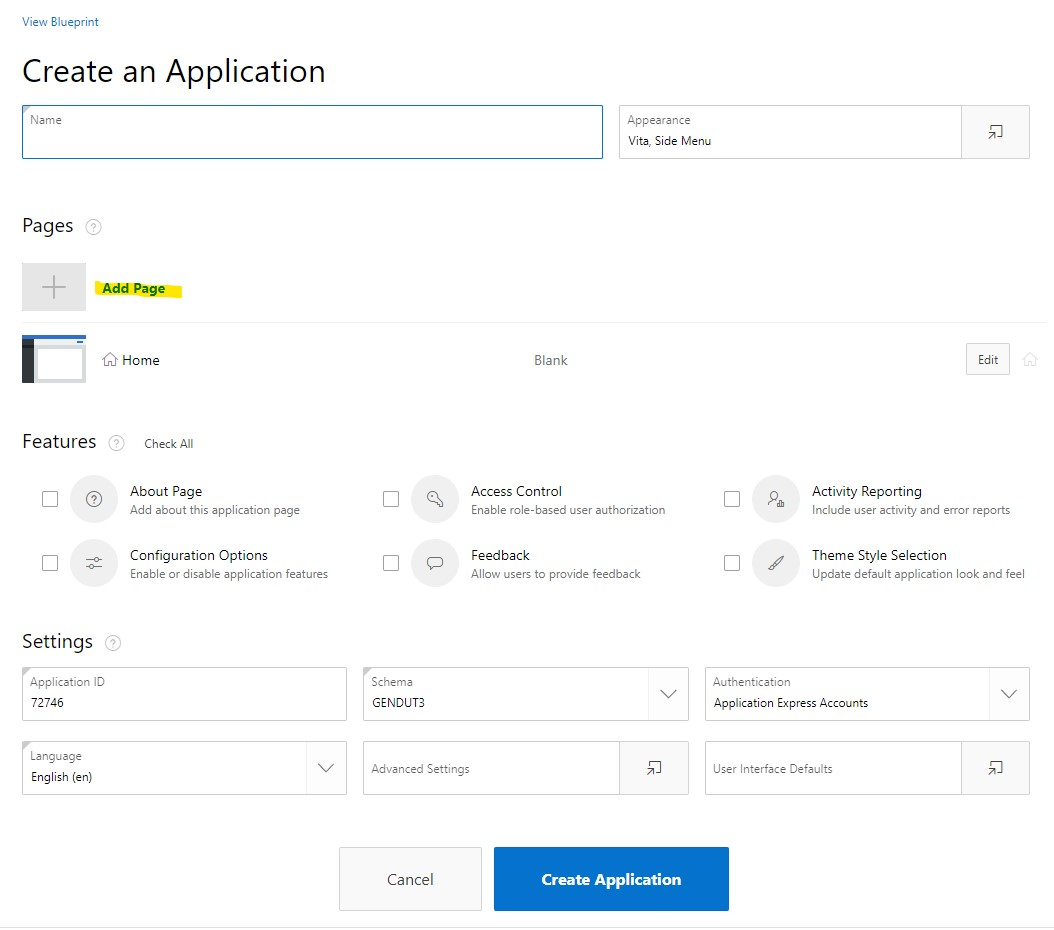
\includegraphics[scale=0.4]{figures/klik_add_page.jpg}
        \caption{\textit{Klik Add Page}}
        \end{center}
        \begin{itemize}
            \item Untuk menambahkan page klik di kolom page, lalu pilih tampilan. Untuk page pertama yaitu query tabel Data Staf, pastikan kalian pilih tampilan sebagai Interactive Report. Lalu masukan nama pagenya setelah itu arahkan ke tabel mana page Interactive Report tersebut. Karena kita ingin melakukan query terhadap tabel Data Staf, maka kita isikan tabelnya adalah Data Staf. 
        \end{itemize}
        \end{figure}
        
        \begin{figure}[!htbp]
        \item[4]Berikut adalah pilihan dari fungsi add page
        \begin{center}
        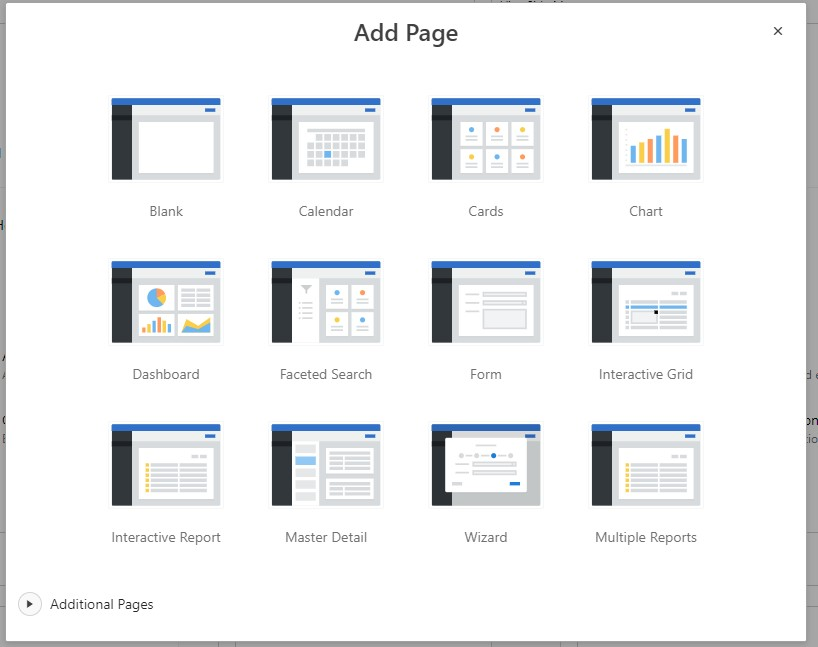
\includegraphics[scale=0.4]{figures/fungsi_add_page.jpg}
        \caption{\textit{Pilihan dari fungsi add page}}
        \end{center}
        \begin{itemize}
            \item Blank = Adalah page yang tidak berisi anda bebas untuk mengisi perlengkapannya seperti item tombol-tombol saat membuat page ini.
            \item Calender = Adalah Page yang berfungsi untuk menambahkan kalender yang di ambil datanya dari database.
            \item Cards = Adalah page yang berisi navigasi untuk membuat item beserta data dari beberapa database.
            \item Charts = Adalah Page yang berisi Laporan yang terstruktur dengan menggunakan chart yang mengambil datanya dari database.
            \item Dashboard = Adalah Page navigasi antara Page atau untuk menampilkan beberapa data atau laporan.
            \item Faceted Search = Adalah Page yang berfungsi untuk search dari Page Lainnya.
            \item Form = Adalah page yang brfungsi untuk membuat form yang nanti akan terisi ke database.
            \item Interactive Grid = Adalah tampilan laporan data dari database.
            \item Interractive Report = Adalah Page untuk menampilkan laporan data yang dapat di edit serta menampilkan hanya beberapa data saja.
            \item Master Detail = Adalah Page yang berfungsi menampilkan data dari database yang telah ternormalisasi seperti relasi antar tabel.
            \item Wizard = Adalah Page untuk menampilkan Form seperti Massage Box atau alert.
            \item Multiple Report = Adalah Page yang berfungsu melihat beberapa report dari tabel database.
        \end{itemize}
        \end{figure}
        
        \begin{figure}[!htbp]
        
        \item[5]Silahkan Pilih Interractive Report
        \begin{center}
        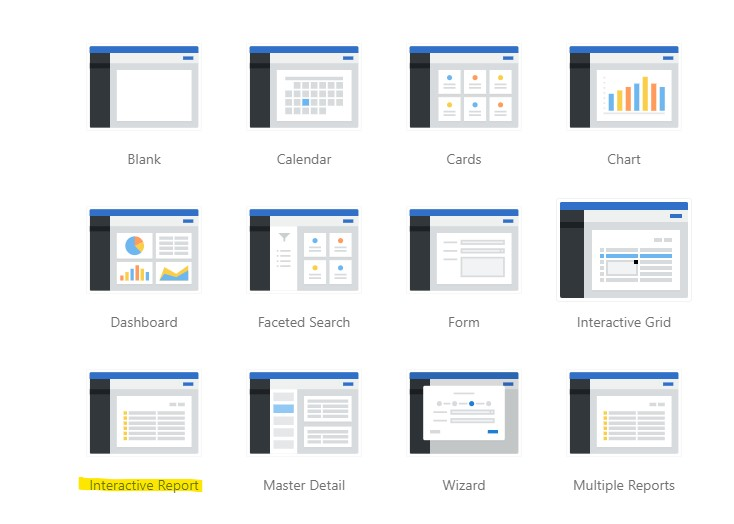
\includegraphics[scale=0.6]{figures/pilih_interractive_report.jpg}
        \caption{\textit{Memilih Interactive Report}}
        \end{center}
                \begin{itemize}
            \item Pilih Interractive Report , mengapa interractive report , agar data dari tabel bisa terstruktur dan  dapat di edit secara langsung dan dapat menampilkan hanya beberapa data yang dibutuhkan
        \end{itemize}
        \end{figure}
        
        \begin{figure}[!htbp]
        \item[6]Anda akan dialihkan ke Add Page Report
        \begin{center}
        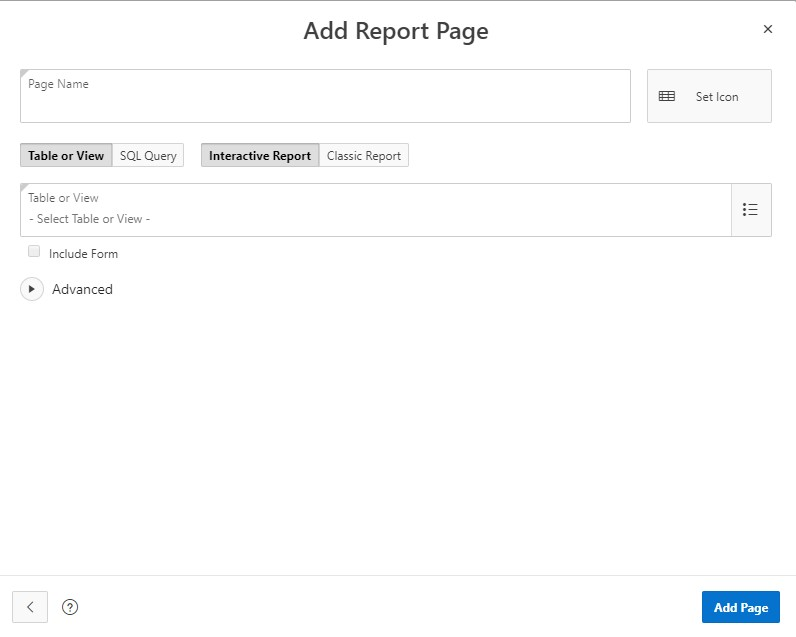
\includegraphics[scale=0.5]{figures/menambahkan_page_report.jpg}
        \caption{\textit{Add Report Page}}
        \end{center}
        \begin{itemize}
            \item Table untuk mengisi kolom yang sudah kita buat tadi
        \end{itemize}
        \end{figure}
        
        \begin{figure}[!htbp]
        \item[7]Ikuti cara berikut kita akan membuat Report Page Beserta Form dari tabel Mahasiswa
        \begin{center}
        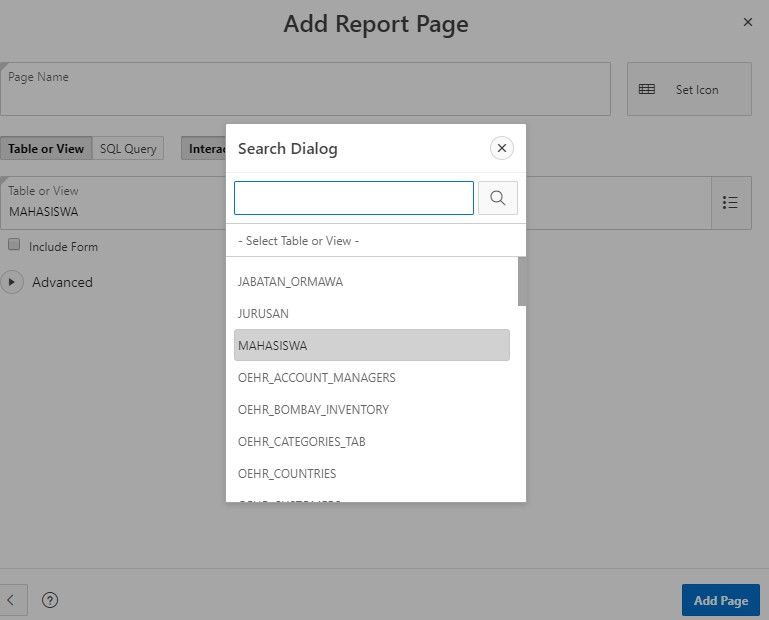
\includegraphics[scale=0.5]{figures/ambil_database_mahasiswa.jpg}
        \caption{\textit{Memilih Tabel Mahasiswa}}
        \end{center}
        \begin{itemize}
            \item Pilih nama mana yang mau anda masukan duluan 
        \end{itemize}
        \end{figure}
        
        \begin{figure}[!htbp]
        \item[8]Lengkapi isian interactive report berikut 
        \begin{center}
        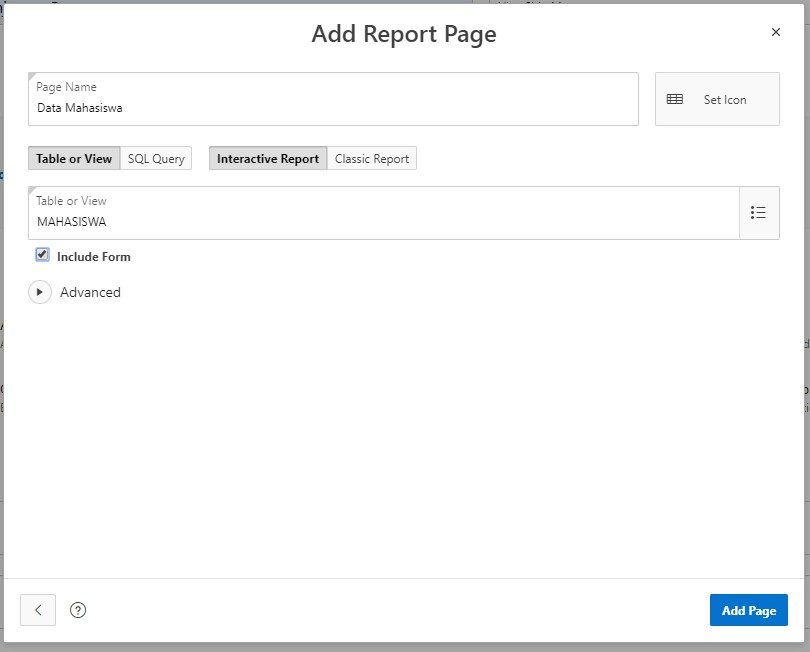
\includegraphics[scale=0.5]{figures/lengkapi_form_interractive.jpg}
        \caption{\textit{Melengkapi Isian Form Interractive}}
        \end{center}
        \begin{itemize}
            \item Pastikan terisi semuanya lalu klik add page  
        \end{itemize}
        \end{figure}
        
        \begin{figure}[!htbp]
        \item[9]Ubah Logo Ikon Pada Page
        \begin{center}
        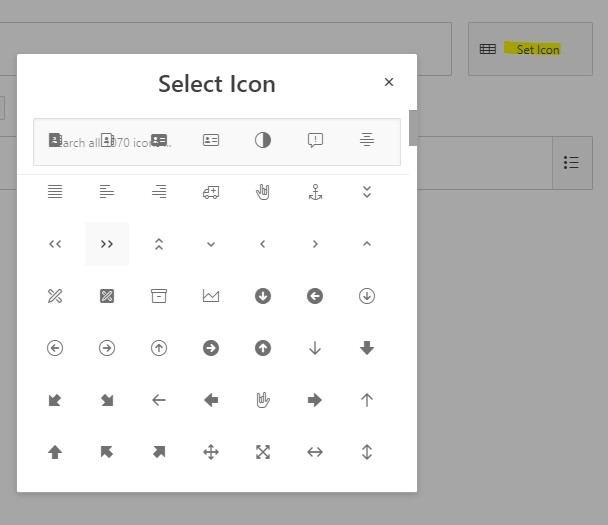
\includegraphics[scale=0.5]{figures/set_icon_interractive.jpg}
        \caption{\textit{Set Icon Page}}
        \end{center}
        \begin{itemize}
            \item pilih ikon yang menurut anda cocok untuk icon table
        \end{itemize}
        \end{figure}
        
        \begin{figure}[!htbp]
        \item[10]Klik Add Page
        \begin{center}
        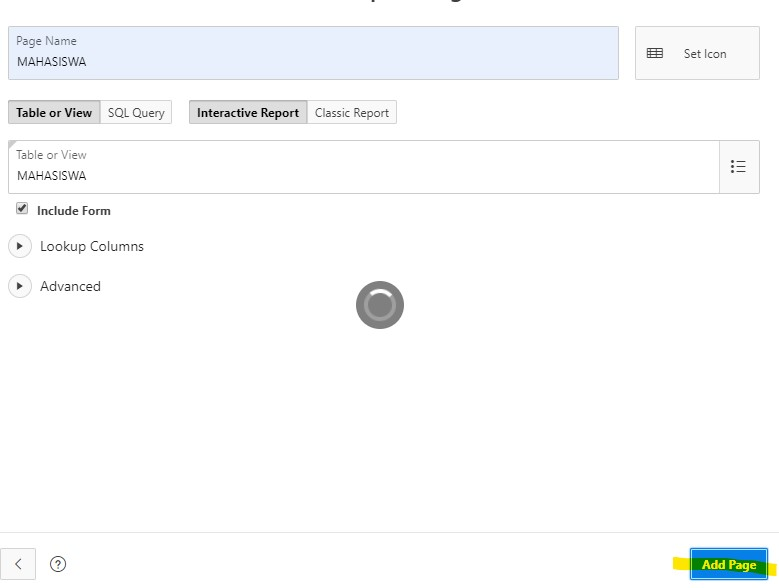
\includegraphics[scale=0.5]{figures/klick_add_page.jpg}
        \caption{\textit{Add Page}}
        \end{center}
       \begin{itemize}
            \item Kalau semua sudah terisi dengan benar lalu add page 
        \end{itemize}
        \end{figure}
        
        \begin{figure}[!htbp]
        \item[11]Untuk Melengkapi Admin silahkan centang features admin berikut
        \begin{center}
        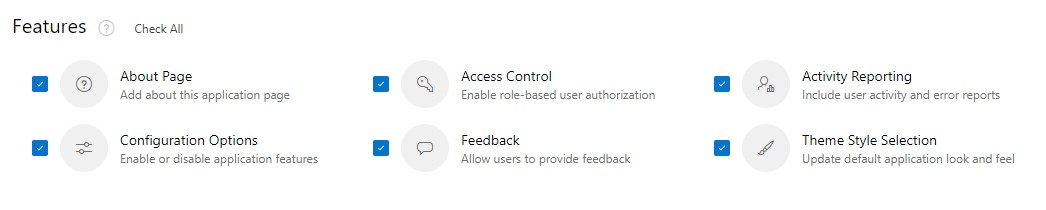
\includegraphics[scale=0.4]{figures/untuk_lengkapi_admin.jpg}
        \caption{\textit{Untuk Melengkapi Admin}}
        \end{center}
        \begin{itemize}
            \item Centang semua FEATURES nya untuk menampilkan pengaturan di aplikasinya 
        \end{itemize}
        \end{figure}
        
        \begin{figure}[!htbp]
        \item[12]Berikut adalah Appearance untuk mengganti tema utama pada aplikasi anda
        \begin{center}
        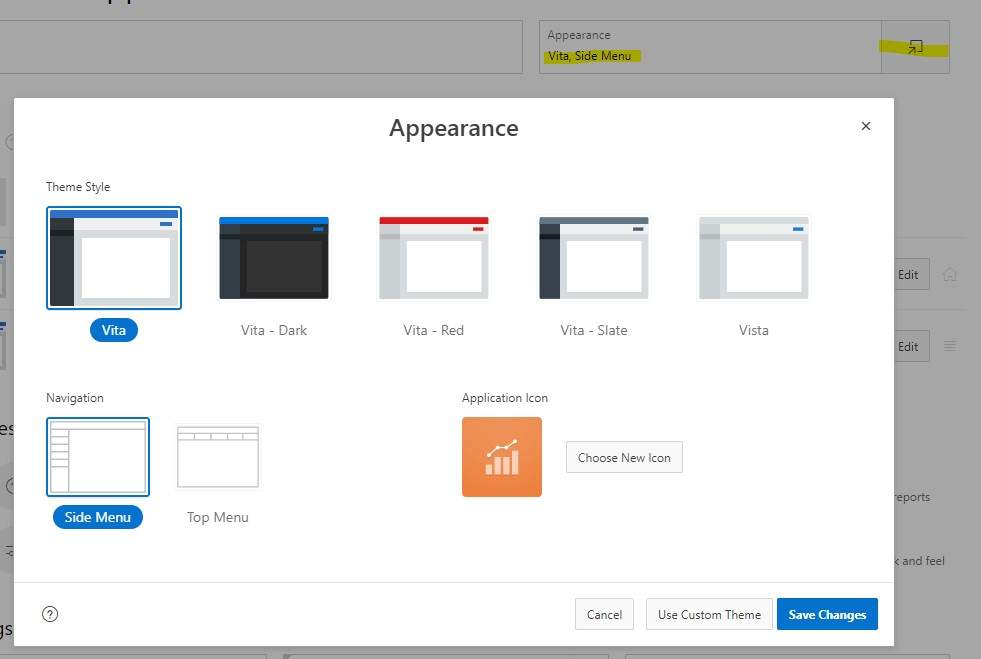
\includegraphics[scale=0.4]{figures/untuk_mengganti_tema.jpg}
        \caption{\textit{Mengganti Tema}}
        \end{center}
        \begin{itemize}
            \item Pilih tema yang menurut anda bagus lalu klik
        \end{itemize}
        \end{figure}
        
        \begin{figure}[!htbp]
        \item[13]Lalu klik Save Changes setelah mengganti tema
        \begin{center}
        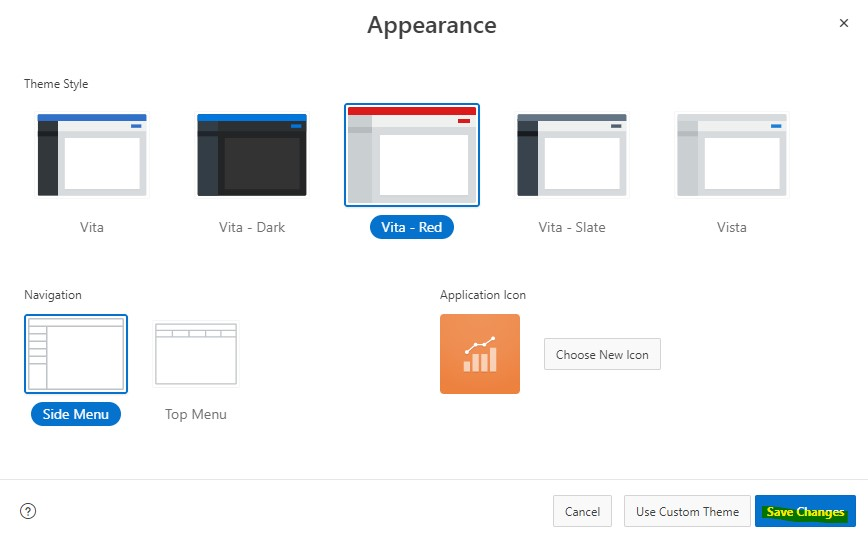
\includegraphics[scale=0.4]{figures/pilih_tema_lalu_klik_save_changes.jpg}
        \caption{\textit{Save Tema}}
        \end{center}
        \begin{itemize}
            \item Setelah anda menganti tema lalu save tema yang telah anda ubah 
        \end{itemize}
        \end{figure}
        
        \begin{figure}[!htbp]
        \item[14]Pastikan Page Master Dibuat Page Master Terdiri (Mahasiswa,Staff Baak, Ruangan, dan Peminjaman Ruangan), ikti cara saat membuat page pada nomer 3 - 10.
        \begin{center}
        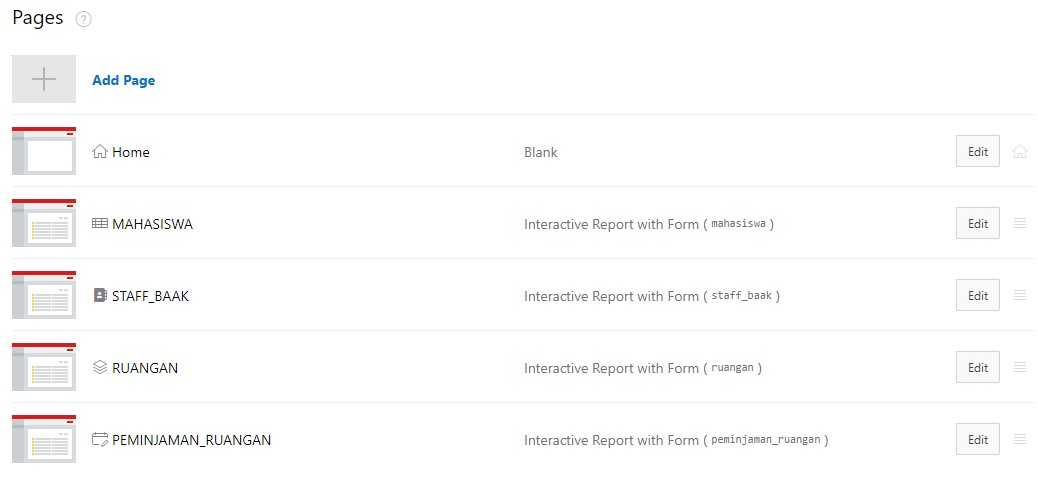
\includegraphics[scale=0.4]{figures/pastikan_page_master_dibuat_terlebih_dahulu.jpg}
        \caption{\textit{Pastikan Page Master Dibuat Terlebih Dahulu}}
        \end{center}
        \end{figure}
        
        \begin{figure}[!htbp]
        \item[15]Setelah sudah pastikan cek dengan lengkap apakah sudah semua
        \begin{center}
        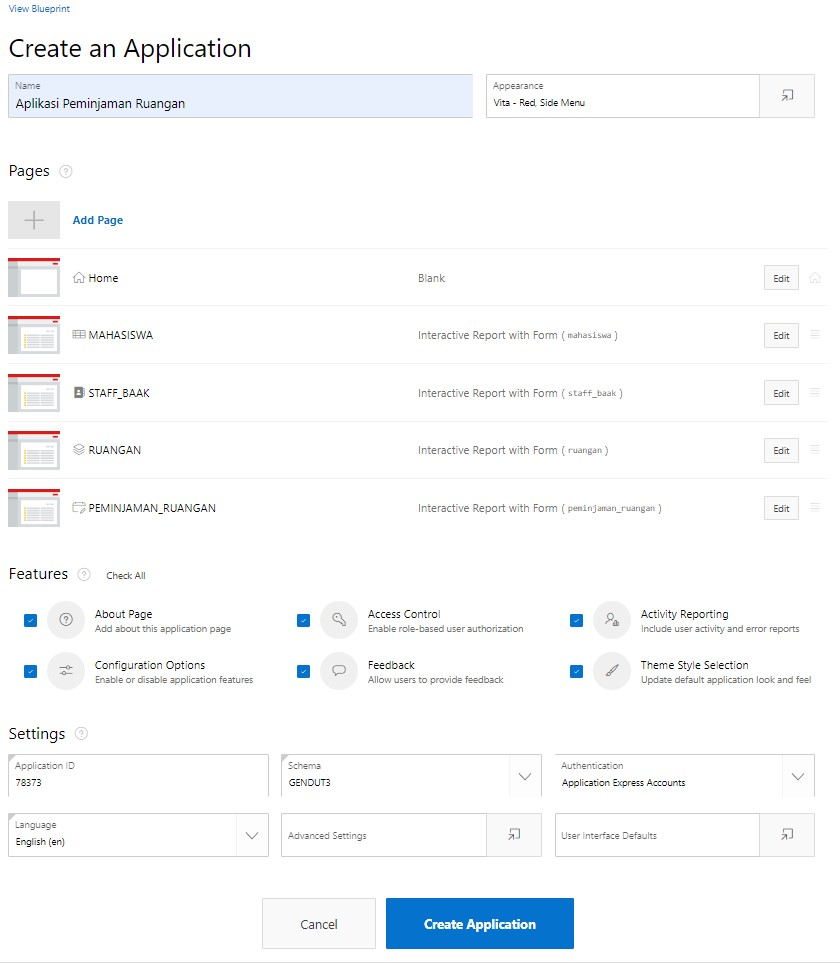
\includegraphics[scale=0.4]{figures/pastikan_sudah_dicek_dan_lengkap.jpg}
        \caption{\textit{Cross Cek Sebelum Di Buat Aplikasi}}
        \end{center}
        \begin{itemize}
            \item Cek kembali semuanya apakah sudah terisi semua dan sudah dicentang semua
        \end{itemize}
        \end{figure}
        
        \begin{figure}[!htbp]
        \item[16]Lalu setelah dirasa sudah klik tombol Create Application
        \begin{center}
        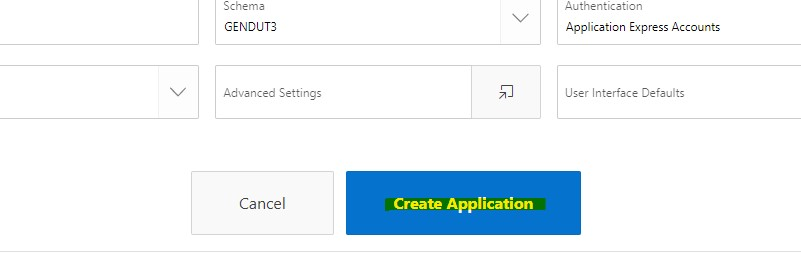
\includegraphics[scale=0.4]{figures/klik_tombol_create_application.jpg}
        \caption{\textit{Klik Create Application}}
        \end{center}   
        \begin{itemize}
            \item CREATE APPLICATION jika anda sudah merasa menggisi semua nya 
        \end{itemize}
        \end{figure}
        
        \begin{figure}[!htbp]
        \item[17]Lalu tunggu loading sejenak untuk proses pembuatan app yang otomatis oleh oracle
        \begin{center}
        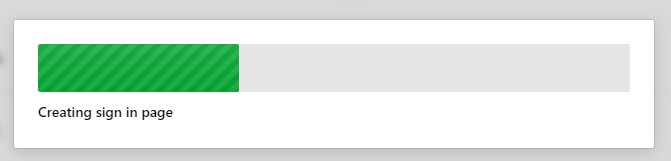
\includegraphics[scale=0.4]{figures/tunggu_loading_app_sdg_dibuat.jpg}
        \caption{\textit{Tunggu Loading App Sedang Dibuat}}
        \end{center}
        \end{figure}
        
        \begin{figure}[!htbp]
        \item[18]Setelah Selesai Anda akan dibawa pada halaman utama Aplikasi anda
        \begin{center}
        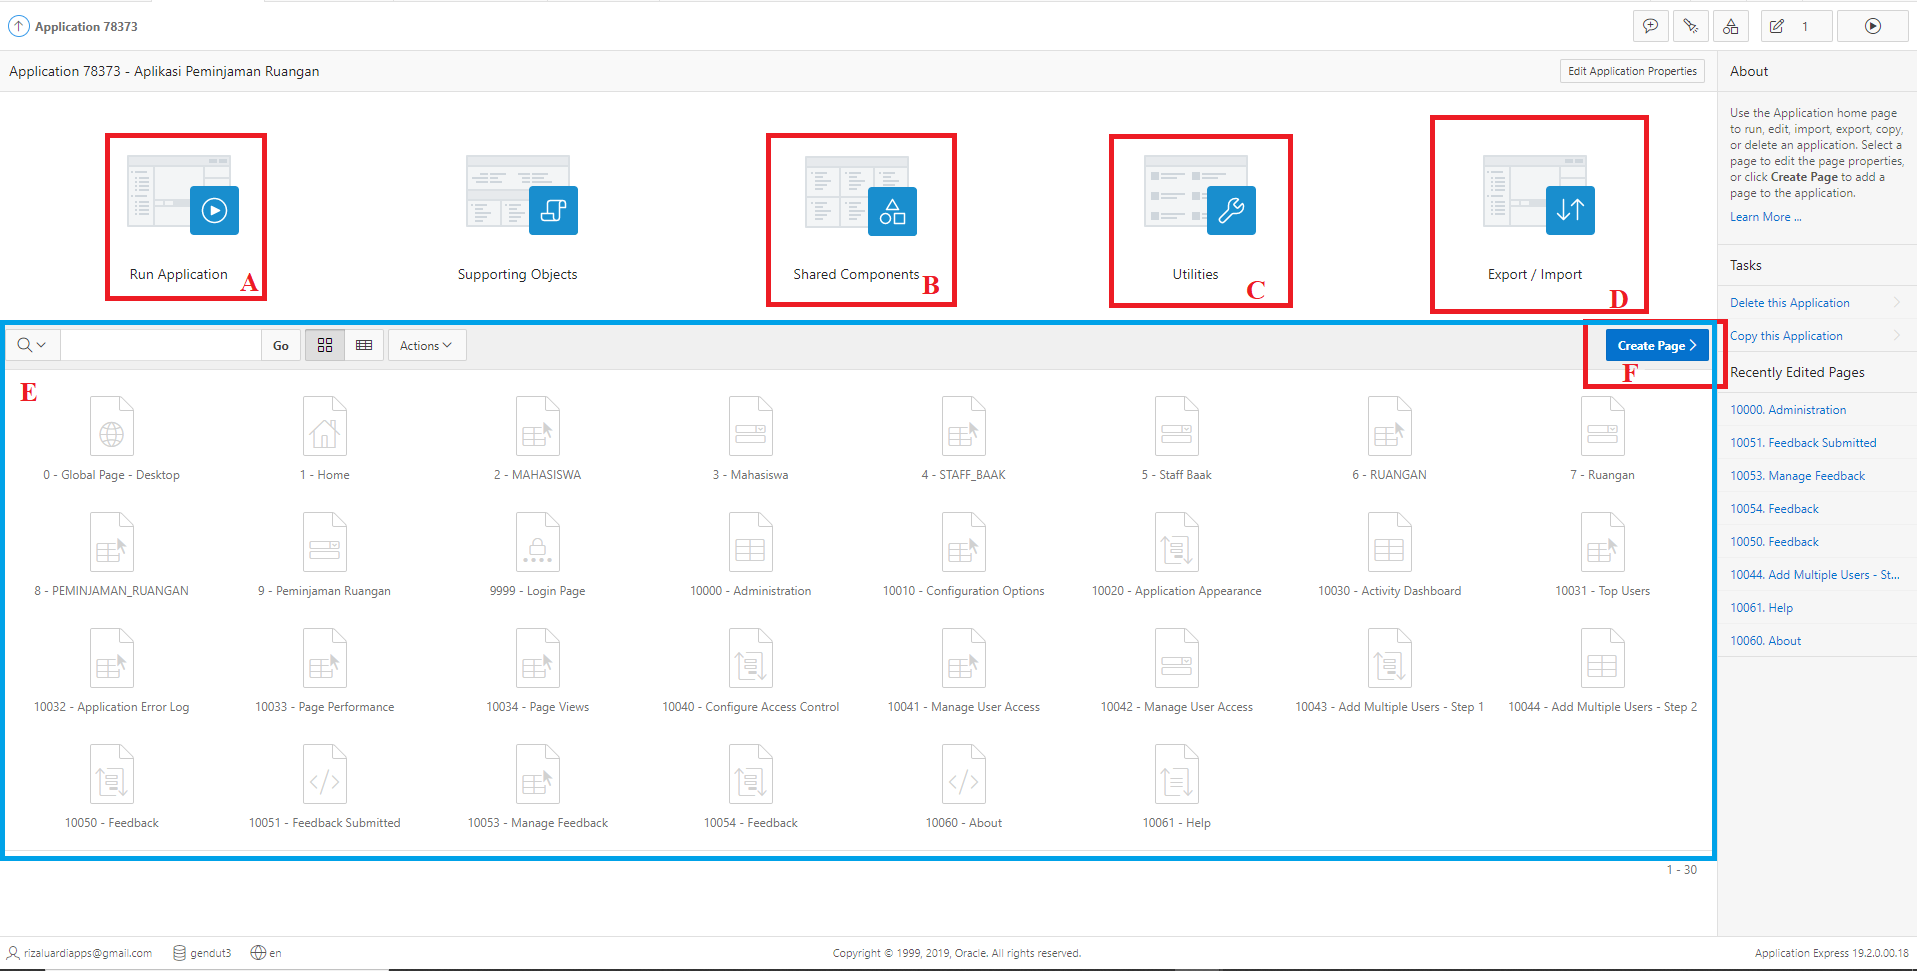
\includegraphics[scale=0.2]{figures/halaman_aplikasi_utiltis.png}
        \caption{\textit{Halaman Utama Apex}}
        \end{center}
        Berikut Penjelasannya
            \begin{itemize}
                \item[A]Untuk Running Aplikasi yang telah dibuat
                \item[B]Shared Components , Berfungsi membuat komponen yang dibutuhkan,nanti yang akan dipakai adalah item list.
                \item[C]Utilities, berfungsi untuk merapihkan halaman tata cara halaman, namun tidak akan dipakai dalam pembuatan aplikasi ini
                \item[D]Export/Import, Berfungsi untuk mengexpor aplikasi menjadikannya sebuah file dan dapat disimpan , lalu untuk memasukkan aplikasi yang telah jadi
                \item[E]Page Aplikasi, berikut adalah Halaman Aplikasi yang telah dibuat tadi sesui urutan pada halaman pertama selalu HOME
                \item[F]Create Page, berfungsi membuat Page Tambahan Pada Aplikasi.
            \end{itemize}
        \end{figure}
        
        \begin{figure}[!htbp]
        \item[19]Pertama kita pilih Run Application, untuk tes aplikasi master yang dibuat tadi, login menggunakan email dan password saat mendaftar
        \begin{center}
        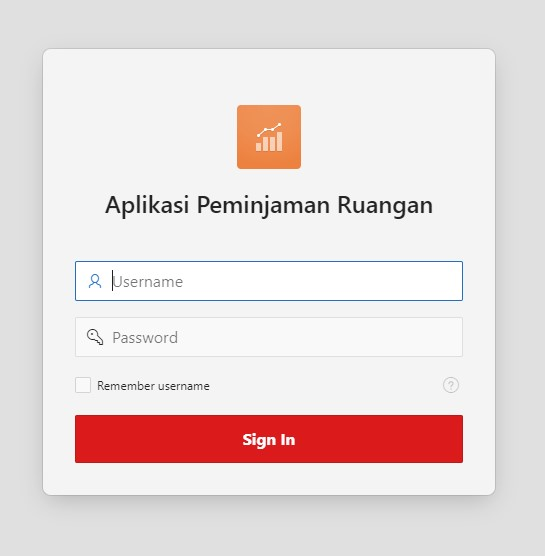
\includegraphics[scale=0.6]{figures/halaman_login_aplikasi.jpg}
        \caption{\textit{Halaman Login Aplikasi}}
        \end{center}
        \end{figure}
        
        \begin{figure}[!htbp]
        \item[20]Berikut adalah tampilan saat di halaman utama Aplikasi
        \begin{center}
        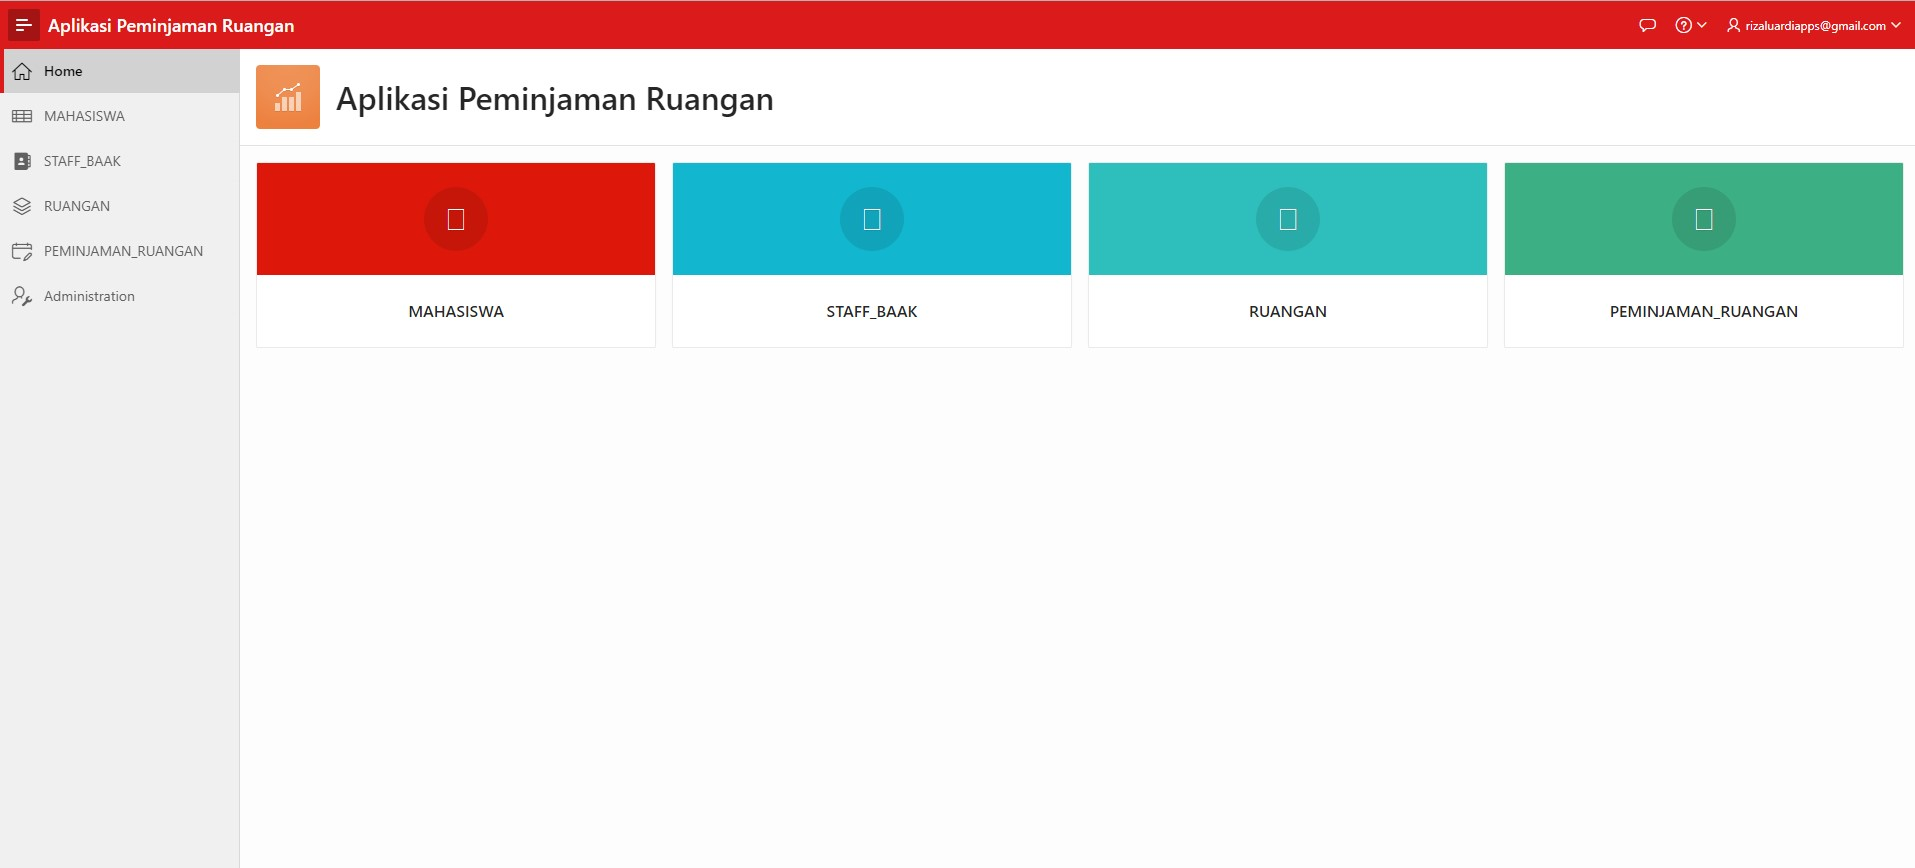
\includegraphics[scale=0.19]{figures/halaman_utm_apps.jpg}
        \caption{\textit{Halaman Utama Aplikasi}}
        \end{center}
        \end{figure}
\end{itemize}


\chapter{Membuat Halaman Baru}
\section{Membuat Halaman Baru Jika Sudah Membuat Halaman Master saat Membuat Aplikasi App Builder}
Berikut cara membuat page baru jika sudah membuat page master , kita akan membuat page ORMAWA,JURUSAN,dan JABATAN\_ORMAWA, kita salah satukan contoh pada ORMAWA.
        \begin{itemize}
        \begin{figure}
        \item[1]Kita Kembali Ke Nomer 18 lalu Pilih Create Page Untuk Membuat Page DATA ORMAWA dan FORM ORMAWA
        \begin{center}
        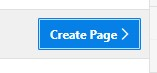
\includegraphics[scale=0.9]{figures/buat_page_baru.jpg}
        \caption{\textit{Create Page}}
        \end{center}
        \end{figure}
        
        \begin{figure}[!htbp]
        \item[2]Lalu Kita Pilih Report Lali Klik Next
        \begin{center}
        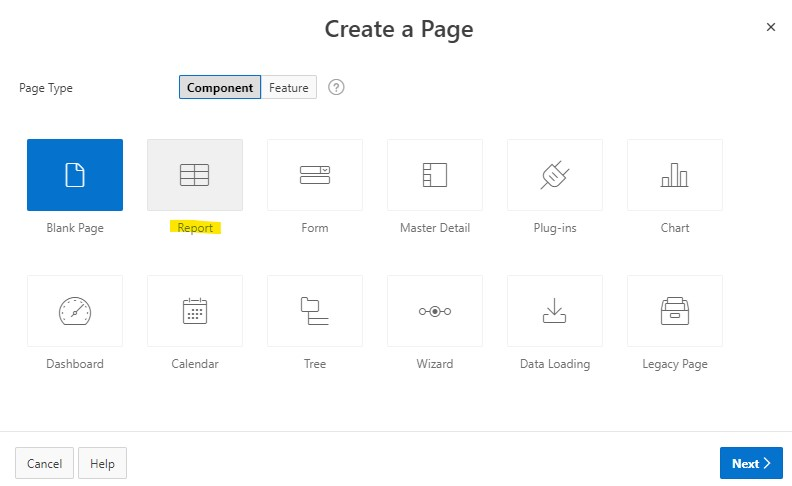
\includegraphics[scale=0.5]{figures/pilih_report.jpg}
        \caption{\textit{Memilih Report}}
        \end{center}
        \end{figure}
        
        \begin{figure}[!htbp]
        \item[3]Pilih Report With Form
        \begin{center}
        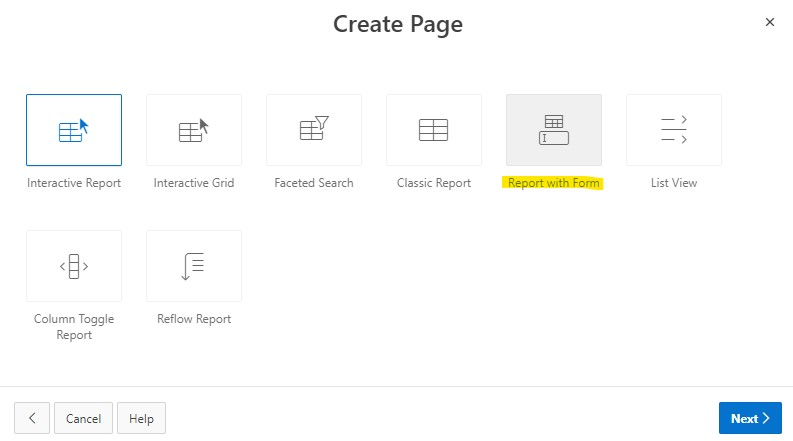
\includegraphics[scale=0.5]{figures/pilih_report_with_form.jpg}
        \caption{\textit{Pilih Report With Form}}
        \end{center}
        \end{figure}
        
        \begin{figure}[!htbp]
        \item[4]Lalu Isi Report Page Name dan Form Page Name Seperti Berikut , abaikan yang lain lalu klik next
        \begin{center}
        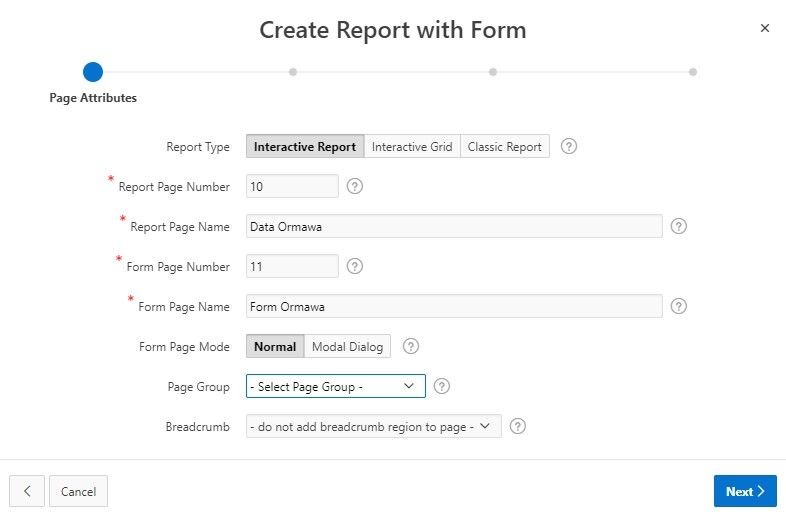
\includegraphics[scale=0.5]{figures/isi_sesuai_kebutuhan_tabel_dan_form_yg_akan_digunakan.jpg}
        \caption{\textit{Create Report With Form}}
        \end{center}
        \end{figure}
        
        \begin{figure}[!htbp]
        \item[5]Lalu pilih Create a new navigation menu entry lalu masukkan pada navigasi mahasiswa
        \begin{center}
        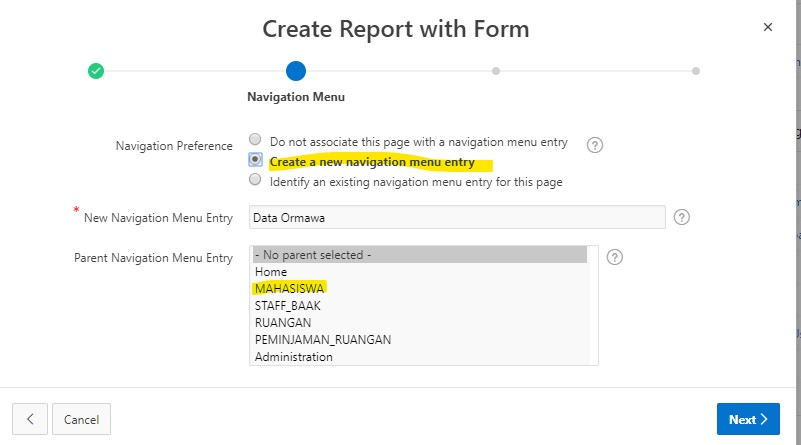
\includegraphics[scale=0.5]{figures/pilih_yang_ditandai.jpg}
        \caption{\textit{Masukan Navigasi}}
        \end{center}
        \end{figure}
        
        \begin{figure}[!htbp]
        \item[6]Pilih Table/View Name isikan tabel Ormawa Yang Telah Dibuat Tadi Lalu Klik Next dan Next Lagi
        \begin{center}
        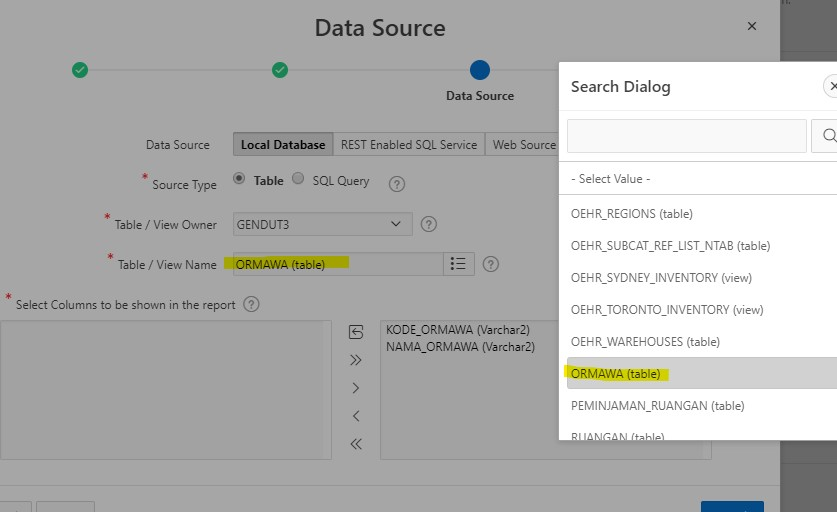
\includegraphics[scale=0.47]{figures/pilih_tabel_ormawa_yg_sudah_dibuat.jpg}
        \caption{\textit{Memilih Tabel Ormawa Dimasukkan pada Page Report Baru}}
        \end{center}
        \end{figure}
        
        \begin{figure}[!htbp]
        \item[7]Setelah terbuat ada 2 Page Ormawa yaitu Data(Untuk Menampilkan Tabel) dan Form Ormawa(untuk menampilakn isian form yang nanti akan diisi ke data tabel), Pertama kita lihat ke Data Ormawa
        \begin{center}
        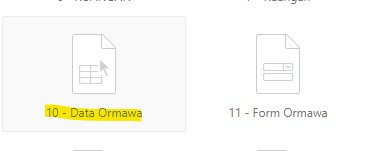
\includegraphics[scale=0.45]{figures/kita_pilih_terlebih_dahulu_data_ormawa.jpg}
        \caption{\textit{Page ORMAWA}}
        \end{center}
        \end{figure}
        
        \begin{figure}[!htbp]
        \item[8]Berikut adalah Halaman Edit Page Designer
        \begin{center}
        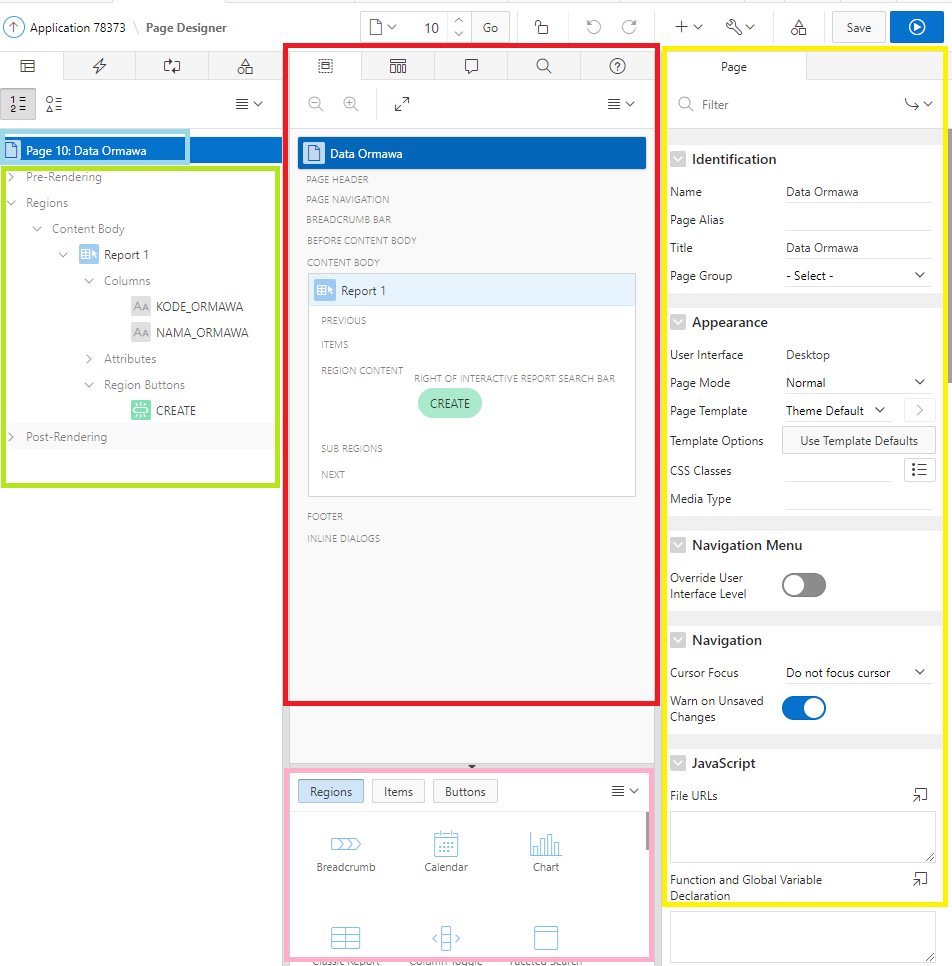
\includegraphics[scale=0.45]{figures/halaman_page_designer.png}
        \caption{\textit{Halaman Edit Page Designer}}
        \end{center}
        Deskripsi
        \begin{itemize}
            \item  HIJAU = Adalah list dari isi page tersebut yang berisi tabel report dari ORMAWA
            \item  MERAH = Adalah isi dari halaman yang akan ditampilkan anda bisa membuat segala macam atribut seperti kalender,box,tombol,chart,dll tinggal seret dari kolom yang ditandai dengan warna merah jambu
        \end{itemize}
        \end{figure}
    
        \begin{figure}[!htbp]
        \begin{itemize}
            \item MERAH JAMBU = adalah isi dari atribut seperti button,text,chart,kalender,breadcumb,bar,dll
            \item KUNING = adalah isi dari page anda bisa mengatunya pada tampilan ini
        \end{itemize}
        \item[9]Sementara pada halaman FORM
        \begin{center}
        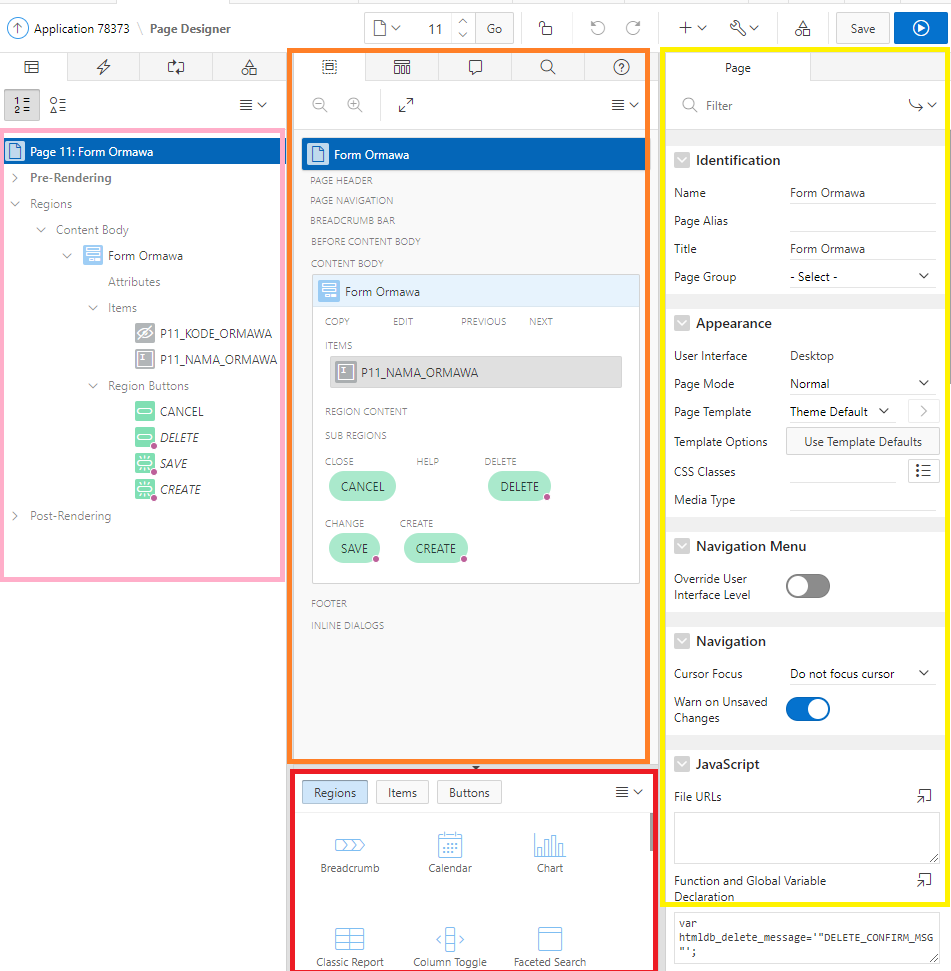
\includegraphics[scale=0.45]{figures/halaman_page_designer_form.png}
        \caption{\textit{Halaman Utama Apex}}
        \end{center}
         \begin{itemize}
            \item  Merah Jambu = Adalah list dari isi page tersebut yang berisi form untuk tabel ORMAWA
            \item  Oranye = Adalah isi dari halaman yang akan ditampilkan anda bisa membuat segala macam atribut seperti kalender,box,tombol,chart,dll tinggal seret dari kolom yang ditandai dengan warna merah jambu
        \end{itemize}
        \end{figure}
        \begin{itemize}
            \item  MERAH = adalah isi dari atribut seperti button,text,chart,kalender,breadcumb,bar,dll.
            \item  KUNING = adalah isi dari page anda bisa mengaturnya segala macam mulai dari proses identifikasi sampai yang lain pada tampilan ini. 
        \end{itemize}
\end{itemize}




\chapter{Membuat Halaman Chart dan Calendar}
\section{Membuat Chart}
Pada aplikasi ini kita akan membuat chart, yaitu chart tentang jurusan yang terbanyak terdata dari tabel jurusan dan mahasiswa.
\begin{itemize}
    \item[1] pertama siapkan terlebih dahulu query View CHART\_JURUSAN seperti berikut :
        \begin{lstlisting}
CREATE OR REPLACE FORCE EDITIONABLE VIEW  "CHART_JURUSAN" ("JURUSAN", "JUMLAH") AS 
  SELECT nama_jurusan, COUNT(nama_jurusan) AS jumlah FROM data_mhs GROUP BY nama_jurusan;        
        \end{lstlisting}
    \item[2] 
\end{itemize}

\section{Membuat Tanggal}

\chapter{Membuat Fungsi Tombol Button}
\section{Membuat Button Dengan Blank Page}
Berikut adalah bab bonus untuk mengaetahui cara membuat Button dan menjalankan dengan sebuah link didalamnya, pada bab selanjutnya akan menggunakan halaman yang sama yaitu TEST PAGE.
\begin{enumerate}\begin{figure}
	\item Pertama tama kita membuat blank page terlebih dahulu pilih blank page, lihat pada Gambar 10.1.
	
        \centering
        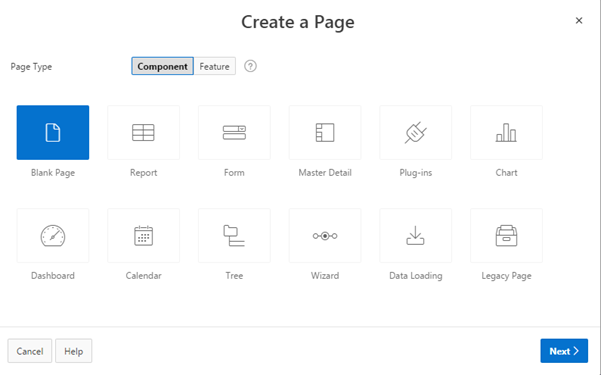
\includegraphics[scale=0.5]{figures/bab10/1.png}
        \caption{\textit{Membuat Blank Page Button}}
        \label{Membuat Blank Page}
    \end{figure}
	\begin{figure}
	\item Kedua beri nama halaman tersebut TEST PAGE, abaikan yang lain lalu klik next, lihat pada Gambar 10.2.
	
        \centering
        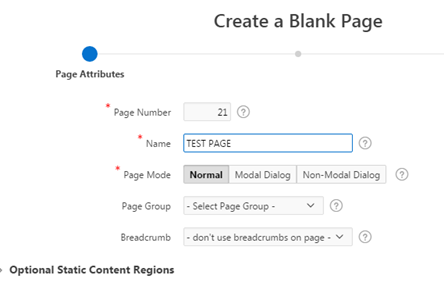
\includegraphics[scale=0.55]{figures/bab10/2.png}
        \caption{\textit{Membuat Blank Page Button 2}}
        \label{Membuat Blank Page 2}
    \end{figure}
	\begin{figure}
	\item Seperti biasa buat navigasi, namun jangan dipilih, kita biarkan default karna akan langsung muncul pada menu navigasi sebelah kiri, lihat pada Gambar 10.3.
	
        \centering
        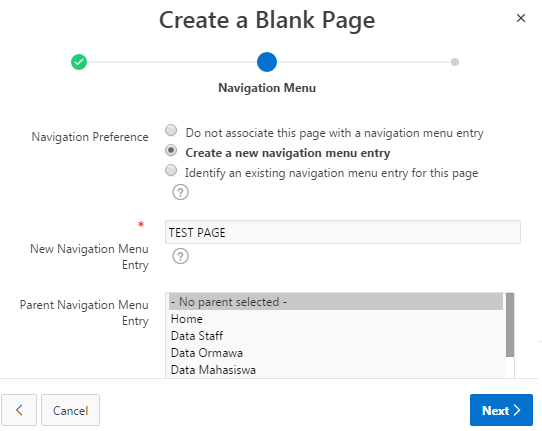
\includegraphics[scale=0.55]{figures/bab10/3.png}
        \caption{\textit{Membuat Blank Page Button 3}}
        \label{Membuat Blank Page 3}
    \end{figure}
    \begin{figure}
	\item Klik finish, lihat pada Gambar 10.4.
	
        \centering
        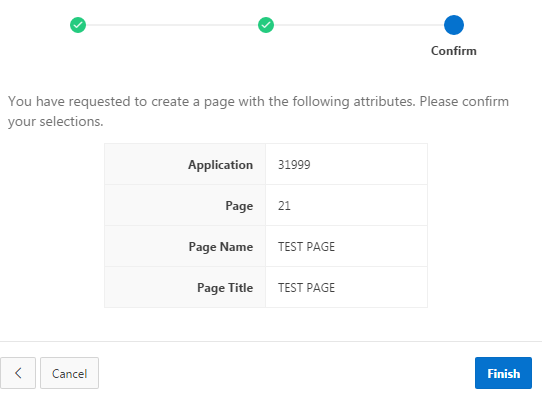
\includegraphics[scale=0.5]{figures/bab10/4.png}
        \caption{\textit{Membuat Blank Page Button 4}}
        \label{Membuat Blank Page 4}
    \end{figure}
	\begin{figure}
	\item Tampilan halaman akan seperti ini, lihat pada Gambar 10.5.
	
        \centering
        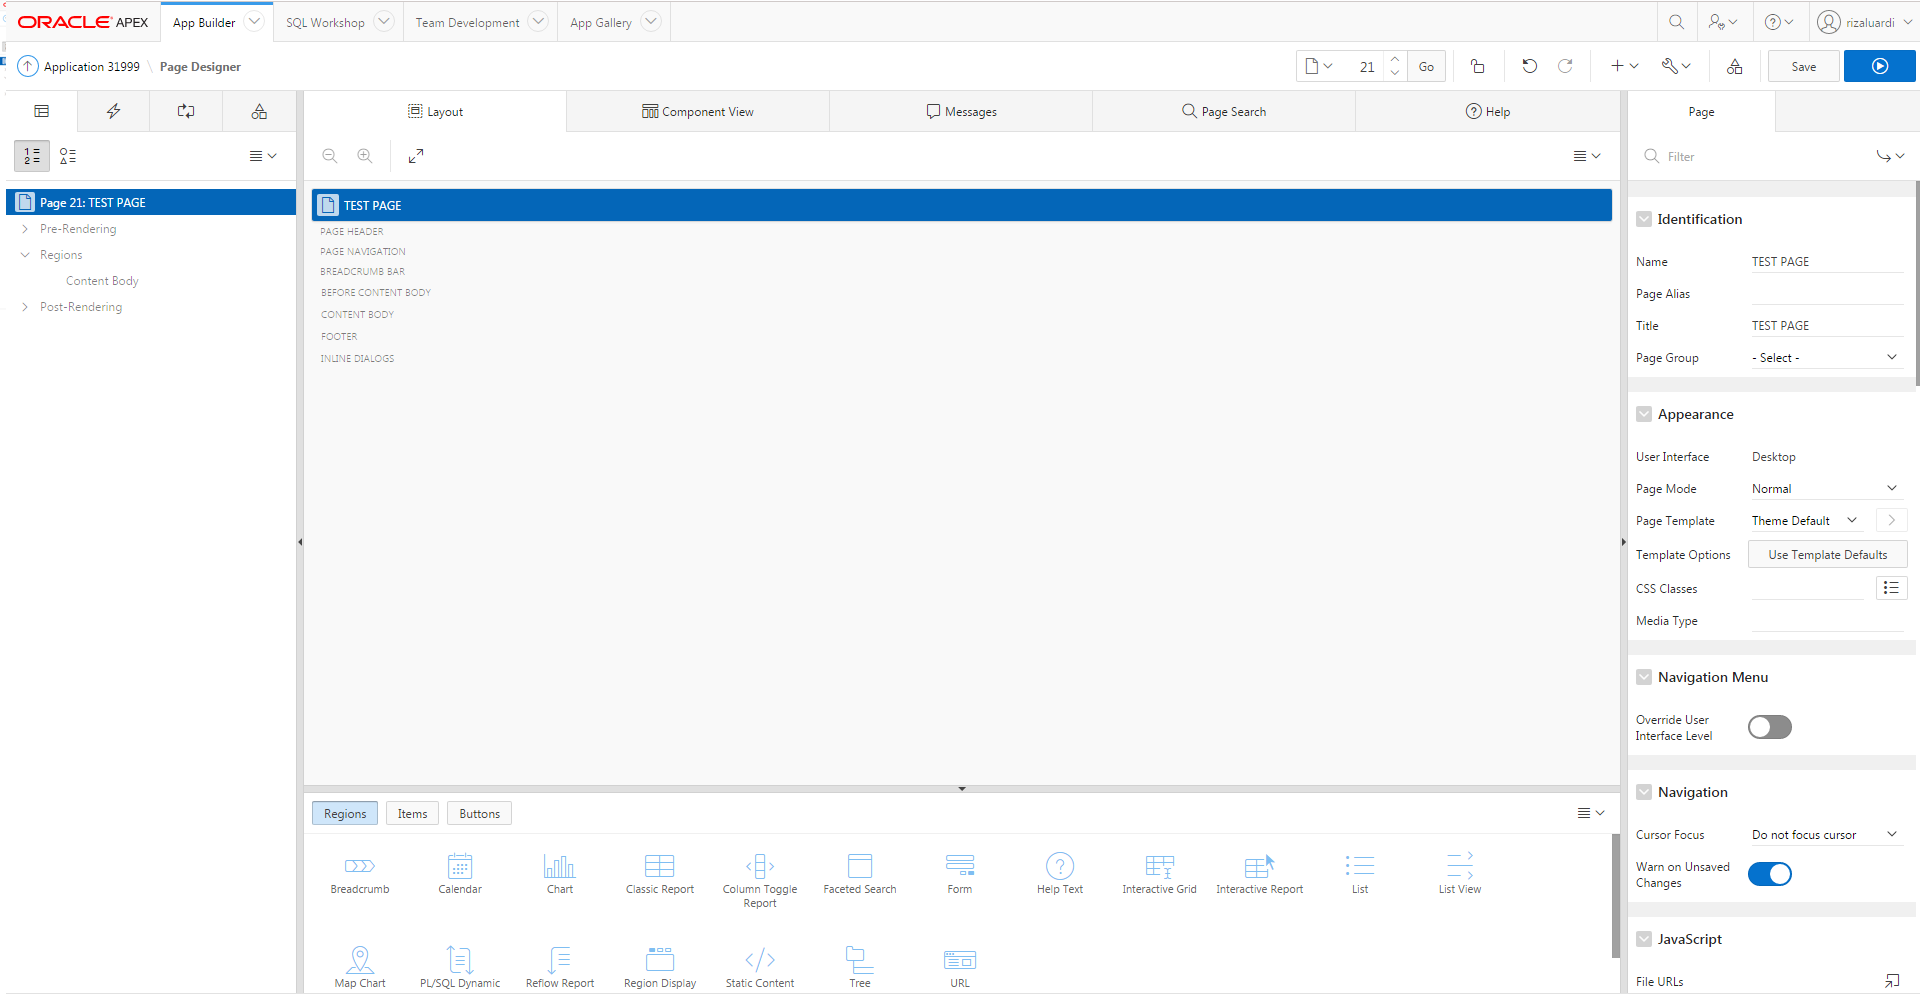
\includegraphics[scale=0.2]{figures/bab10/5.png}
        \caption{\textit{Tampilan Blank Page}}
        \label{}
    \end{figure}
    \begin{figure}
    \item Untuk membuat button pertama kita pilih pda tab regions Breadcumb lalu tarik ke Content Body, lihat pada Gambar 10.6.
	
        \centering
        \includegraphics[scale=0.4]{figures/bab10/6.png}
        \caption{\textit{Pilih Breadcumb}}
        \label{Pilih Breadcumb}
    \end{figure}
    
	\begin{figure}
	\item Pada navigasi oracle sebelah kanan terlihat ada Identification dan Source pilih Type dan Breadcumb menjadi Breadcumb, lihat pada Gambar 10.7.
	
        \centering
        \includegraphics[scale=0.7]{figures/bab10/7.png}
        \caption{\textit{Identification Breadcumb}}
        \label{Identification Breadcumb}
    \end{figure}
	\begin{figure}
	\item pada item button di navigasi bawah ada 6 macam tipe button ada dengan icon,hot icon,text,hot text,text dengan icon,dan text dengan icon hot, lihat pada Gambar 10.8.
	
        \centering
        \includegraphics[scale=0.55]{figures/bab10/8.png}
        \caption{\textit{Macam Jenis Icon}}
        \label{Macam Jenis Icon}
    \end{figure}
	\begin{figure}
	\item tarik button text pada item page, lihat pada Gambar 10.9.
	
        \centering
        \includegraphics[scale=0.22]{figures/bab10/15.png}
        \caption{\textit{Memasukkan Button pada Breadcumb}}
        \label{Memasukkan Button Pada Breadcumb}
    \end{figure}
	\begin{figure}
	\item Isi Identification dengan Nama, pastikan Button Name tidak diberi spasi atau gunakan Underscore untuk memberi jark antara huruf, beri nama Label untuk agar terlihat pada User Interface Aplikasi, lihat pada Gambar 10.10.
	
        \centering
        \includegraphics[scale=0.7]{figures/bab10/9.png}
        \caption{\textit{Identification Button}}
        \label{Identification Button}
    \end{figure}
    \begin{figure}
	\item Di bawahnya Identification ada Tab Behavior pilih action menjadi Redirect To Url, lihat pada Gambar 10.11.
	
        \centering
        \includegraphics[scale=0.7]{figures/bab10/10.png}
        \caption{\textit{Behavior Button}}
        \label{Behavior Button}
    \end{figure}
    \begin{figure}
	\item klik link target No Link Defined, lihat pada Gambar 10.12.
	
        \centering
        \includegraphics[scale=0.7]{figures/bab10/11.png}
        \caption{\textit{Link Target}}
        \label{Link Target}
    \end{figure}
	\begin{figure}
	\item isikan link target button contoh github.com/rizaluardi lalu klik ok dan save, lihat pada Gambar 10.13.
	
        \centering
        \includegraphics[scale=0.65]{figures/bab10/12.png}
        \caption{\textit{Link Target 2}}
        \label{Link Target 2}
    \end{figure}
	\begin{figure}
	\item hasilnya akan seperti berikut, lihat pada Gambar 10.14.
	
        \centering
        \includegraphics[scale=0.5]{figures/bab10/13.png}
        \caption{\textit{Hasil Button}}
        \label{Hasil Button}
    \end{figure}
	\begin{figure}
	\item anda juga bisa memberi button dengan icon, lihat pada Gambar 10.15.

        \centering
        \includegraphics[scale=0.25]{figures/bab10/14.png}
        \caption{\textit{Button Icon}}
        \label{Button Icon}
    \end{figure}

\end{enumerate}

 






\chapter{Membuat Fungsi Static Contents Dengan HTML dan CSS}
Dalam pembuatan aplikasi Oracle Apex Online, anda juga dapat memodifikasi source HTML dan CSS yang anda inginkan untuk mempercantik antarmuka penggunaan aplikasi.
\section{Pengertian HTML}
Hypertext Markup Language adalah sebuah bahasa pemrograman yang diciptakan untuk membuat program tampilan halaman web dasar, pada HTML juga terdiri dari beberapa kode yang biasa diawali dengan kurung siku buka dan diakhiri dengan kurung siku tutup.
\par dalam program HTML sangatlah sederhana tidak serumit dengan PHP atau bahasa lainnya, HTML berguna untuk menciptakan Interface atau Antarmuka pengguna dengan aplikasi web, biasanya bidang FRONT-end Developer saja yang ditugaskan untuk merancang aplikasi namun.
\par HTML juga ada beberapa jenis, misalnya HTML5 yaitu web antarmuka yang Responsive dengan segala macam device baik dari komputer,laptop,sampai pada mobile device, HTML5 biasanya ditambahkan dengan Bootstrap JS(Javascript) maupun Bootstrap CSS(Cascading Style Sheet) yaitu perantara agar dapat memberikan antarmuka yang sempurna dalam membuat web HTML5
\par Adapun kode sederhana yang dipakai dalam penggunaan bahasa HTML sebagai berikut:
\begin{lstlisting}
<!DOCTYPE html>
<html>
<head>
<title>Titel Halaman</title>
</head>
<body>

<h1>Ini adalah heading</h1>
<p>Ini adalah Paragraf.</p>

</body>
</html>
\end{lstlisting}

\section{Pengertian CSS}
Cascading Style Sheet adalah sebuah perantara bahasa pemrograman yang digunakan untuk menambahkan atribut pada kode HTML, dalam pembuatan HTML biasanya menggunakan CSS yang berguna untuk mempercantik atau mempermudah interaksi dengan pengguna website.
\par Dalam CSS juga anda dapat mengatur atribut dan juga fungsi-fungsi yang digunakan pada kode HTML misalkan memperbaiki tampilan, mengubah warna, memperbaiki tata letak sebuah kode seperti div page, dan banyak lagi.
\par Kode sederhana CSS yang digunakan pada HTML adalah sebagai berikut:
\begin{lstlisting}
<!DOCTYPE html>
<html>
<head>
<style>
body {background-color: green;}
h1   {color: blue;}
p    {color: red;}
</style>
</head>
<body>

<h1>Ini adalah heading</h1>
<p>Ini adalah paragraf.</p>

</body>
</html>
\end{lstlisting}

\par Untuk menyatukannya kita menggunakan script HTML dan CSS, kita akan membuat sebuah STATIC CONTENT tentang halaman About Us, yang dimana menampil-kan profil kami pada sebuah halaman website, kodenya seperti berikut:

\begin{lstlisting}
<style type="text/css">
#kiri
{
width:50%;
height:100%;
float:left;
}
#kanan
{
width:50%;
height:100%;
float:right;
}
img{
border-radius:70%;
}
</style>

<div id="kiri"><center>
  <h3>Rizaluardi Achmad Pratama</h3>
  <p>1184102
  <p><img width="25%" height="25%" src="...isi dengan source gambar....">

</center></div>

<div id="kanan"><center>
    <h3>M Ichsam Kurniawan Nasution</h3>
    <p>1184110
    <p><img width="25%" height="25%" src="....isi dengan source gambar...">
</center></div>
\end{lstlisting}

\par berikut adalah contoh dari kode CSS yang tergabung dalam HTML, buatlah kode tersebut untuk mengetahui step selanjutnya.

\section{Menggabungkan HTML dengan CSS dan Memasukan pada Aplikasi}
Untuk memasukkannya kita ikuti langkah langkah berikut :
\begin{enumerate}
    
    \begin{figure}
	\item Buatlah STATIC CONTENT pada halaman TEST PAGE yang sudah dibuat sebelumnya, anda bisa menemukannya pada Regions lalu pilih Static Content, lihat pada Gambar 11.1.
	
        \centering
        \includegraphics[scale=0.5]{figures/bab11/1.png}
        \caption{\textit{Static Content}}
        \label{Static Content}
    \end{figure}
    
    \begin{figure}
    \item Tarik Static Content menuju Content Body , lihat pada Gambar 11.2.
        
        \centering
        \includegraphics[scale=0.5]{figures/bab11/2.png}
        \caption{\textit{Static Content 2}}
        \label{Static Content 2}
    \end{figure}
    
    \begin{figure}
    \item Lalu buatlah title dengan nama About Us, setelah itu pada menu source akan terlihar text, disitulah yang nantinya akan dimasukkan kode dari HTML dan CSS klik tombol yang ditandai warna merah, lihat pada Gambar 11.3.
    
        \centering
        \includegraphics[scale=0.5]{figures/bab11/3.png}
        \caption{\textit{Static Content 3}}
        \label{Static Content 3}
    \end{figure}
    
    \begin{figure}
    \item Lalu masukkan kode yang telah dibuat tadi ke Code Editor berikut pastikan isikan source gambar yang anda inginkan, lihat pada Gambar 11.4.
        
        \centering
        \includegraphics[scale=0.5]{figures/bab11/4.png}
        \caption{\textit{Static Content 4}}
        \label{Static Content4}
    \end{figure}
    
    \begin{figure}
    \item Berikut adalah Tampilan jika kita memasukkan HTML dan CSS pada aplikasi Oracle Apex menggunakan Static Content, lihat pada Gambar 11.5.
        
        \centering
        \includegraphics[scale=0.4]{figures/bab11/5.png}
        \caption{\textit{Hasil Static Content}}
        \label{Static Content5}
    \end{figure}
    
    
\end{enumerate}

\chapter{Membuat Fungsi URL Dengan Website Lain}
\section{Pendahuluan}
Dalam fungsi URL yaitu untuk menampilkan sebuah website dalam website oracle apex, mungkin penjelasannya masih bingung, jadi seperti ini, dalam halaman oracle misalkan halaman TEST PAGE yang kita buat lalu kita akan membuat sebuah page di dalam halaman tersebut page tersebut berisikan halaman yang muncul dari URL lain, seperti halnya iFrame pada HTML.

\par IFRAME merupakan sebuah tag html yang berfungsi untuk menampilkan halaman website tanpa harus membuka halaman baru pada browser, pengguna akan disajikan halaman yang sudah ada seperti membuka website di dalam website.

\par Dalam penggunaan di oracle apex iframe dapat ditemukan pada tab Region yaitu URL yang dimana kita hanya memasukkan URL yang akan ditampilkan pada suatu halaman di oracle APEX tersebut.

\par Berikut adalah cara untuk membuat iFrame pada Oracle Apex:

\begin{enumerate}
\begin{figure}
    \item Pertama kita lihat pada tab regions lalu kita pilih URL, lihat pada Gambar 11.1.
        
        \centering
        \includegraphics[scale=0.5]{figures/bab12/1.png}
        \caption{\textit{URL iFrame}}
        \label{URL iFrame}
    \end{figure}
    
    \begin{figure}
    \item Kemudian tarik dan lepaskan pada Content Body dibawah Test Page, lihat pada Gambar 11.2.
        
        \centering
        \includegraphics[scale=0.5]{figures/bab12/2.png}
        \caption{\textit{URL iFrame 2}}
        \label{URL iFrame 2}
    \end{figure}
    
    \begin{figure}
    \item Pada tab Identification kita beri Nama Title, lihat pada Gambar 11.3.
        
        \centering
        \includegraphics[scale=0.5]{figures/bab12/3.png}
        \caption{\textit{URL iFrame 3}}
        \label{URL iFrame 3}
    \end{figure}
    
    \begin{figure}
    \item Selanjutnya lihat pada menu navigasi di sebelah kiri klik Attributes yang sudah ditandai dengan warna merah dan bulatan hitam, lihat pada Gambar 11.4.
        
        \centering
        \includegraphics[scale=0.5]{figures/bab12/4.png}
        \caption{\textit{URL iFrame 4}}
        \label{URL iFrame 4}
    \end{figure}
    
    \begin{figure}
    \item Lalu masukkan URL salah satu website contoh \textit{https://if.poltekpos.ac.id} lalu masukan IFrame Attributes yaitu atribut dari iframe misalkan tinggi dan lebar IFrame yang diinginkan, lihat pada Gambar 11.5.
        
        \centering
        \includegraphics[scale=0.5]{figures/bab12/5.png}
        \caption{\textit{URL iFrame 5}}
        \label{URL iFrame 5}
    \end{figure}
    
    \begin{figure}
    \item Klik save dan bila sudah di Run akan menampilkan halaman seperti berikut, lihat pada Gambar 11.6.
        
        \centering
        \includegraphics[scale=0.22]{figures/bab12/6.png}
        \caption{\textit{URL iFrame 6}}
        \label{URL iFrame 6}
    \end{figure}
    
    
\end{enumerate}
 



\bibliographystyle{IEEEtran} 
%\def\bibfont{\normalsize}
\bibliography{references}


%%%%%%%%%%%%%%%
%%  The default LaTeX Index
%%  Don't need to add any commands before \begin{document}

%%%% Making an index
%% 
%% 1. Make index entries, don't leave any spaces so that they
%% will be sorted correctly.
%% 
%% \index{term}
%% \index{term!subterm}
%% \index{term!subterm!subsubterm}
%% 
%% 2. Run LaTeX several times to produce <filename>.idx
%% 
%% 3. On command line, type  makeindx <filename> which
%% will produce <filename>.ind 
%% 
%% 4. Type \printindex to make the index appear in your book.
%% 
%% 5. If you would like to edit <filename>.ind 
%% you may do so. See docs.pdf for more information.
%% 
%%%%%%%%%%%%%%%%%%%%%%%%%%%%%%

%%%%%%%%%%%%%% Making Multiple Indices %%%%%%%%%%%%%%%%
%% 1. 
%% \usepackage{multind}
%% \makeindex{book}
%% \makeindex{authors}
%% \begin{document}
%% 
%% 2.
%% % add index terms to your book, ie,
%% \index{book}{A term to go to the topic index}
%% \index{authors}{Put this author in the author index}
%% 
%% \index{book}{Cows}
%% \index{book}{Cows!Jersey}
%% \index{book}{Cows!Jersey!Brown}
%% 
%% \index{author}{Douglas Adams}
%% \index{author}{Boethius}
%% \index{author}{Mark Twain}
%% 
%% 3. On command line type 
%% makeindex topic 
%% makeindex authors
%% 
%% 4.
%% this is a Wiley command to make the indices print:
%% \multiprintindex{book}{Topic index}
%% \multiprintindex{authors}{Author index}

\end{document}


